%&preformat-disser
\RequirePackage[l2tabu,orthodox]{nag} % Раскомментировав, можно в логе получать рекомендации относительно правильного использования пакетов и предупреждения об устаревших и нерекомендуемых пакетах
% Формат А4, 14pt (ГОСТ Р 7.0.11-2011, 5.3.6)
\documentclass[a4paper,14pt,oneside,openany]{memoir}

%%%%%%%%%%%%%%%%%%%%%%%%%%%%%%%%%%%%%%%%%%%%%%%%%%%%%%%%%%%%%%%%%%%%%%%%%%%%%%%%
%%%% Файл упрощённых настроек шаблона, общих для диссертации и автореферата %%%%
%%%%%%%%%%%%%%%%%%%%%%%%%%%%%%%%%%%%%%%%%%%%%%%%%%%%%%%%%%%%%%%%%%%%%%%%%%%%%%%%

%%% Режим черновика %%%
\makeatletter
\@ifundefined{c@draft}{
  \newcounter{draft}
  \setcounter{draft}{0}  % 0 --- чистовик (максимальное соблюдение ГОСТ)
  % 1 --- черновик (отклонения от ГОСТ, но быстрая
  %       сборка итоговых PDF)
}{}
\makeatother

%%% Пометки в тексте %%%
\makeatletter
\@ifundefined{c@showmarkup}{
  \newcounter{showmarkup}
  \setcounter{showmarkup}{1}  % 0 --- скрыть пометки
  % 1 --- показывать пометки
}{}
\makeatother

%%% Использование в pdflatex шрифтов не по-умолчанию %%%
\makeatletter
\@ifundefined{c@usealtfont}{
  \newcounter{usealtfont}
  \setcounter{usealtfont}{1}    % 0 --- шрифты на базе Computer Modern
  % 1 --- использовать пакет pscyr, при его
  %       наличии
  % 2 --- использовать пакет XCharter, при наличии
  %       подходящей версии
}{}
\makeatother

%%% Использование в xelatex и lualatex семейств шрифтов %%%
\makeatletter
\@ifundefined{c@fontfamily}{
  \newcounter{fontfamily}
  \setcounter{fontfamily}{1}  % 0 --- CMU семейство. Используется как fallback;
  % 1 --- Шрифты от MS (Times New Roman и компания)
  % 2 --- Семейство Liberation
}{}
\makeatother

%%% Библиография %%%
\makeatletter
\@ifundefined{c@bibliosel}{
  \newcounter{bibliosel}
  \setcounter{bibliosel}{1}   % 0 --- встроенная реализация с загрузкой файла
  %       через движок bibtex8;
  % 1 --- реализация пакетом biblatex через движок
  %       biber
}{}
\makeatother

%%% Вывод типов ссылок в библиографии %%%
\makeatletter
\@ifundefined{c@mediadisplay}{
  \newcounter{mediadisplay}
  \setcounter{mediadisplay}{1}   % 0 --- не делать ничего; надписи [Текст] и
  %       [Эл. ресурс] будут выводиться только в ссылках с
  %       заполненным полем `media`;
  % 1 --- автоматически добавлять надпись [Текст] к ссылкам с
  %       незаполненным полем `media`; таким образом, у всех
  %       источников будет указан тип, что соответствует
  %       требованиям ГОСТ
  % 2 --- автоматически удалять надписи [Текст], [Эл. Ресурс] и др.;
  %       не соответствует ГОСТ
  % 3 --- автоматически удалять надпись [Текст];
  %       не соответствует ГОСТ
  % 4 --- автоматически удалять надпись [Эл. Ресурс];
  %       не соответствует ГОСТ
}{}
\makeatother

%%% Предкомпиляция tikz рисунков для ускорения работы %%%
\makeatletter
\@ifundefined{c@imgprecompile}{
  \newcounter{imgprecompile}
  \setcounter{imgprecompile}{0}   % 0 --- без предкомпиляции;
  % 1 --- пользоваться предварительно
  %       скомпилированными pdf вместо генерации
  %       заново из tikz
}{}
\makeatother
            % общие настройки шаблона
\input{common/packages}         % Пакеты общие для диссертации и автореферата
\synopsisfalse                      % Этот документ --- не автореферат
\input{Dissertation/dispackages}    % Пакеты для диссертации
\input{Dissertation/userpackages}   % Пакеты для специфических пользовательских задач

%%%%%%%%%%%%%%%%%%%%%%%%%%%%%%%%%%%%%%%%%%%%%%%%%%%%%%
%%%% Файл упрощённых настроек шаблона диссертации %%%%
%%%%%%%%%%%%%%%%%%%%%%%%%%%%%%%%%%%%%%%%%%%%%%%%%%%%%%

%%% Инициализирование переменных, не трогать!  %%%
\newcounter{intvl}
\newcounter{otstup}
\newcounter{contnumeq}
\newcounter{contnumfig}
\newcounter{contnumtab}
\newcounter{pgnum}
\newcounter{chapstyle}
\newcounter{headingdelim}
\newcounter{headingalign}
\newcounter{headingsize}
%%%%%%%%%%%%%%%%%%%%%%%%%%%%%%%%%%%%%%%%%%%%%%%%%%%%%%

%%% Область упрощённого управления оформлением %%%

%% Интервал между заголовками и между заголовком и текстом %%
% Заголовки отделяют от текста сверху и снизу
% тремя интервалами (ГОСТ Р 7.0.11-2011, 5.3.5)
\setcounter{intvl}{3}               % Коэффициент кратности к размеру шрифта

%% Отступы у заголовков в тексте %%
\setcounter{otstup}{0}              % 0 --- без отступа; 1 --- абзацный отступ

%% Нумерация формул, таблиц и рисунков %%
% Нумерация формул
\setcounter{contnumeq}{0}   % 0 --- пораздельно (во введении подряд,
%       без номера раздела);
% 1 --- сквозная нумерация по всей диссертации
% Нумерация рисунков
\setcounter{contnumfig}{0}  % 0 --- пораздельно (во введении подряд,
%       без номера раздела);
% 1 --- сквозная нумерация по всей диссертации
% Нумерация таблиц
\setcounter{contnumtab}{1}  % 0 --- пораздельно (во введении подряд,
%       без номера раздела);
% 1 --- сквозная нумерация по всей диссертации

%% Оглавление %%
\setcounter{pgnum}{1}       % 0 --- номера страниц никак не обозначены;
% 1 --- Стр. над номерами страниц (дважды
%       компилировать после изменения настройки)
\settocdepth{subsection}    % до какого уровня подразделов выносить в оглавление
\setsecnumdepth{subsection} % до какого уровня нумеровать подразделы


%% Текст и форматирование заголовков %%
\setcounter{chapstyle}{1}     % 0 --- разделы только под номером;
% 1 --- разделы с названием "Глава" перед номером
\setcounter{headingdelim}{1}  % 0 --- номер отделен пропуском в 1em или \quad;
% 1 --- номера разделов и приложений отделены
%       точкой с пробелом, подразделы пропуском
%       без точки;
% 2 --- номера разделов, подразделов и приложений
%       отделены точкой с пробелом.

%% Выравнивание заголовков в тексте %%
\setcounter{headingalign}{0}  % 0 --- по центру;
% 1 --- по левому краю

%% Размеры заголовков в тексте %%
\setcounter{headingsize}{0}   % 0 --- по ГОСТ, все всегда 14 пт;
% 1 --- пропорционально изменяющийся размер
%       в зависимости от базового шрифта

%% Подпись таблиц %%

% Смещение строк подписи после первой строки
\newcommand{\tabindent}{0cm}

% Тип форматирования заголовка таблицы:
% plain --- название и текст в одной строке
% split --- название и текст в разных строках
\newcommand{\tabformat}{plain}

%%% Настройки форматирования таблицы `plain`

% Выравнивание по центру подписи, состоящей из одной строки:
% true  --- выравнивать
% false --- не выравнивать
\newcommand{\tabsinglecenter}{false}

% Выравнивание подписи таблиц:
% justified   --- выравнивать как обычный текст («по ширине»)
% centering   --- выравнивать по центру
% centerlast  --- выравнивать по центру только последнюю строку
% centerfirst --- выравнивать по центру только первую строку (не рекомендуется)
% raggedleft  --- выравнивать по правому краю
% raggedright --- выравнивать по левому краю
\newcommand{\tabjust}{justified}

% Разделитель записи «Таблица #» и названия таблицы
\newcommand{\tablabelsep}{~\cyrdash\ }

%%% Настройки форматирования таблицы `split`

% Положение названия таблицы:
% \centering   --- выравнивать по центру
% \raggedleft  --- выравнивать по правому краю
% \raggedright --- выравнивать по левому краю
\newcommand{\splitformatlabel}{\raggedleft}

% Положение текста подписи:
% \centering   --- выравнивать по центру
% \raggedleft  --- выравнивать по правому краю
% \raggedright --- выравнивать по левому краю
\newcommand{\splitformattext}{\raggedright}

%% Подпись рисунков %%
%Разделитель записи «Рисунок #» и названия рисунка
\newcommand{\figlabelsep}{~\cyrdash\ }  % (ГОСТ 2.105, 4.3.1)
% "--- здесь не работает

%%% Цвета гиперссылок %%%
% Latex color definitions: http://latexcolor.com/
\definecolor{linkcolor}{rgb}{0.9,0,0}
\definecolor{citecolor}{rgb}{0,0.6,0}
\definecolor{urlcolor}{rgb}{0,0,1}
%\definecolor{linkcolor}{rgb}{0,0,0} %black
%\definecolor{citecolor}{rgb}{0,0,0} %black
%\definecolor{urlcolor}{rgb}{0,0,0} %black
      % Упрощённые настройки шаблона

\input{common/newnames}         % Новые переменные, для всего проекта

%%% Основные сведения %%%
\newcommand{\thesisAuthorLastName}{Ильев}
\newcommand{\thesisAuthorOtherNames}{Сергей Викторович}
\newcommand{\thesisAuthorInitials}{С.\,В.}
\newcommand{\thesisAuthor}             % Диссертация, ФИО автора
{%
    \texorpdfstring{% \texorpdfstring takes two arguments and uses the first for (La)TeX and the second for pdf
        \thesisAuthorLastName~\thesisAuthorOtherNames% так будет отображаться на титульном листе или в тексте, где будет использоваться переменная
    }{%
        \thesisAuthorLastName, \thesisAuthorOtherNames% эта запись для свойств pdf-файла. В таком виде, если pdf будет обработан программами для сбора библиографических сведений, будет правильно представлена фамилия.
    }
}
\newcommand{\thesisAuthorShort}        % Диссертация, ФИО автора инициалами
{\thesisAuthorInitials~\thesisAuthorLastName}
%\newcommand{\thesisUdk}                % Диссертация, УДК
%{\fixme{xxx.xxx}}
\newcommand{\thesisTitle}              % Диссертация, название
{Исследование микроскопической природы функциональных свойств ячеек сегнетоэлектрической памяти на основе тонких плёнок оксида гафния-циркония}
\newcommand{\thesisSpecialtyNumber}    % Диссертация, специальность, номер
{03.03.01}
\newcommand{\thesisSpecialtyTitle}     % Диссертация, специальность, название (название взято с сайта ВАК для примера)
{Прикладные математика и физика}
%% \newcommand{\thesisSpecialtyTwoNumber} % Диссертация, вторая специальность, номер
%% {\fixme{XX.XX.XX}}
%% \newcommand{\thesisSpecialtyTwoTitle}  % Диссертация, вторая специальность, название
%% {\fixme{Теория и~методика физического воспитания, спортивной тренировки,
%% оздоровительной и~адаптивной физической культуры}}
\newcommand{\thesisDegree}             % Диссертация, ученая степень
{\fixme{кандидата физико-математических наук}}
\newcommand{\thesisDegreeShort}        % Диссертация, ученая степень, краткая запись
{\fixme{канд. физ.-мат. наук}}
\newcommand{\thesisCity}               % Диссертация, город написания диссертации
{Долгопрудный}
\newcommand{\thesisYear}               % Диссертация, год написания диссертации
{\the\year}
\newcommand{\thesisOrganization}       % Диссертация, организация
{Федеральное государственное автономное образовательное учреждение высшего образования <<Московский физико-технический институт (национальный исследовательский университет)>>}
\newcommand{\thesisOrganizationShort}  % Диссертация, краткое название организации для доклада
{\fixme{НазУчДисРаб}}

\newcommand{\thesisInOrganization}     % Диссертация, организация в предложном падеже: Работа выполнена в ...
{\fixme{учреждении с~длинным длинным длинным длинным названием, в~котором
        выполнялась данная диссертационная работа}}

%% \newcommand{\supervisorDead}{}           % Рисовать рамку вокруг фамилии
\newcommand{\supervisorFio}              % Научный руководитель, ФИО
{Чуприк Анастасия Александровна}
\newcommand{\supervisorRegalia}          % Научный руководитель, регалии
{к.ф.-м.н., доцент}
% \newcommand{\supervisorFioShort}         % Научный руководитель, ФИО
% {\fixme{И.\,О.~Фамилия}}
% \newcommand{\supervisorRegaliaShort}     % Научный руководитель, регалии
% {\fixme{уч.~ст.,~уч.~зв.}}

%% \newcommand{\supervisorTwoDead}{}        % Рисовать рамку вокруг фамилии
%% \newcommand{\supervisorTwoFio}           % Второй научный руководитель, ФИО
%% {\fixme{Фамилия Имя Отчество}}
%% \newcommand{\supervisorTwoRegalia}       % Второй научный руководитель, регалии
%% {\fixme{уч. степень, уч. звание}}
%% \newcommand{\supervisorTwoFioShort}      % Второй научный руководитель, ФИО
%% {\fixme{И.\,О.~Фамилия}}
%% \newcommand{\supervisorTwoRegaliaShort}  % Второй научный руководитель, регалии
%% {\fixme{уч.~ст.,~уч.~зв.}}

\newcommand{\opponentOneFio}           % Оппонент 1, ФИО
{\fixme{Фамилия Имя Отчество}}
\newcommand{\opponentOneRegalia}       % Оппонент 1, регалии
{\fixme{доктор физико-математических наук, профессор}}
\newcommand{\opponentOneJobPlace}      % Оппонент 1, место работы
{\fixme{Не очень длинное название для места работы}}
\newcommand{\opponentOneJobPost}       % Оппонент 1, должность
{\fixme{старший научный сотрудник}}

\newcommand{\opponentTwoFio}           % Оппонент 2, ФИО
{\fixme{Фамилия Имя Отчество}}
\newcommand{\opponentTwoRegalia}       % Оппонент 2, регалии
{\fixme{кандидат физико-математических наук}}
\newcommand{\opponentTwoJobPlace}      % Оппонент 2, место работы
{\fixme{Основное место работы c длинным длинным длинным длинным названием}}
\newcommand{\opponentTwoJobPost}       % Оппонент 2, должность
{\fixme{старший научный сотрудник}}

%% \newcommand{\opponentThreeFio}         % Оппонент 3, ФИО
%% {\fixme{Фамилия Имя Отчество}}
%% \newcommand{\opponentThreeRegalia}     % Оппонент 3, регалии
%% {\fixme{кандидат физико-математических наук}}
%% \newcommand{\opponentThreeJobPlace}    % Оппонент 3, место работы
%% {\fixme{Основное место работы c длинным длинным длинным длинным названием}}
%% \newcommand{\opponentThreeJobPost}     % Оппонент 3, должность
%% {\fixme{старший научный сотрудник}}

\newcommand{\leadingOrganizationTitle} % Ведущая организация, дополнительные строки. Удалить, чтобы не отображать в автореферате
{\fixme{Федеральное государственное бюджетное образовательное учреждение высшего
        профессионального образования с~длинным длинным длинным длинным названием}}

\newcommand{\defenseDate}              % Защита, дата
{\fixme{DD mmmmmmmm YYYY~г.~в~XX часов}}
\newcommand{\defenseCouncilNumber}     % Защита, номер диссертационного совета
{\fixme{Д\,123.456.78}}
\newcommand{\defenseCouncilTitle}      % Защита, учреждение диссертационного совета
{\fixme{Название учреждения}}
\newcommand{\defenseCouncilAddress}    % Защита, адрес учреждение диссертационного совета
{\fixme{Адрес}}
\newcommand{\defenseCouncilPhone}      % Телефон для справок
{\fixme{+7~(0000)~00-00-00}}

\newcommand{\defenseSecretaryFio}      % Секретарь диссертационного совета, ФИО
{\fixme{Фамилия Имя Отчество}}
\newcommand{\defenseSecretaryRegalia}  % Секретарь диссертационного совета, регалии
{\fixme{д-р~физ.-мат. наук}}            % Для сокращений есть ГОСТы, например: ГОСТ Р 7.0.12-2011 + http://base.garant.ru/179724/#block_30000

\newcommand{\synopsisLibrary}          % Автореферат, название библиотеки
{\fixme{Название библиотеки}}
\newcommand{\synopsisDate}             % Автореферат, дата рассылки
{\fixme{DD mmmmmmmm}\the\year~года}

% To avoid conflict with beamer class use \providecommand
\providecommand{\keywords}%            % Ключевые слова для метаданных PDF диссертации и автореферата
{}
             % Основные сведения
\input{common/fonts}            % Определение шрифтов (частичное)
%%% Шаблон %%%
\DeclareRobustCommand{\fixme}{\textcolor{red}}  % решаем проблему превращения
% названия цвета в результате \MakeUppercase,
% http://tex.stackexchange.com/a/187930,
% \DeclareRobustCommand protects \fixme
% from expanding inside \MakeUppercase
\AtBeginDocument{%
    \setlength{\parindent}{2.5em}                   % Абзацный отступ. Должен быть одинаковым по всему тексту и равен пяти знакам (ГОСТ Р 7.0.11-2011, 5.3.7).
}

%%% Таблицы %%%
\DeclareCaptionLabelSeparator{tabsep}{\tablabelsep} % нумерация таблиц
\DeclareCaptionFormat{split}{\splitformatlabel#1\par\splitformattext#3}

\captionsetup[table]{
    format=\tabformat,                % формат подписи (plain|hang)
    font=normal,                      % нормальные размер, цвет, стиль шрифта
    skip=.0pt,                        % отбивка под подписью
    parskip=.0pt,                     % отбивка между параграфами подписи
    position=above,                   % положение подписи
    justification=\tabjust,           % центровка
    indent=\tabindent,                % смещение строк после первой
    labelsep=tabsep,                  % разделитель
    singlelinecheck=\tabsinglecenter, % не выравнивать по центру, если умещается в одну строку
}

%%% Рисунки %%%
\DeclareCaptionLabelSeparator{figsep}{\figlabelsep} % нумерация рисунков

\captionsetup[figure]{
    format=plain,                     % формат подписи (plain|hang)
    font=normal,                      % нормальные размер, цвет, стиль шрифта
    skip=.0pt,                        % отбивка под подписью
    parskip=.0pt,                     % отбивка между параграфами подписи
    position=below,                   % положение подписи
    singlelinecheck=true,             % выравнивание по центру, если умещается в одну строку
    justification=centerlast,         % центровка
    labelsep=figsep,                  % разделитель
}

%%% Подписи подрисунков %%%
\DeclareCaptionSubType{figure}
\renewcommand\thesubfigure{\asbuk{subfigure}} % нумерация подрисунков
\ifsynopsis
    \DeclareCaptionFont{norm}{\fontsize{10pt}{11pt}\selectfont}
    \newcommand{\subfigureskip}{2.pt}
\else
    \DeclareCaptionFont{norm}{\fontsize{14pt}{16pt}\selectfont}
    \newcommand{\subfigureskip}{0.pt}
\fi

\captionsetup[subfloat]{
    labelfont=norm,                 % нормальный размер подписей подрисунков
    textfont=norm,                  % нормальный размер подписей подрисунков
    labelsep=space,                 % разделитель
    labelformat=brace,              % одна скобка справа от номера
    justification=centering,        % центровка
    singlelinecheck=true,           % выравнивание по центру, если умещается в одну строку
    skip=\subfigureskip,            % отбивка над подписью
    parskip=.0pt,                   % отбивка между параграфами подписи
    position=below,                 % положение подписи
}

%%% Настройки ссылок на рисунки, таблицы и др. %%%
% команды \cref...format отвечают за форматирование при помощи команды \cref
% команды \labelcref...format отвечают за форматирование при помощи команды \labelcref

\ifpresentation
\else
    \crefdefaultlabelformat{#2#1#3}

    % Уравнение
    \crefformat{equation}{(#2#1#3)} % одиночная ссылка с приставкой
    \labelcrefformat{equation}{(#2#1#3)} % одиночная ссылка без приставки
    \crefrangeformat{equation}{(#3#1#4) \cyrdash~(#5#2#6)} % диапазон ссылок с приставкой
    \labelcrefrangeformat{equation}{(#3#1#4) \cyrdash~(#5#2#6)} % диапазон ссылок без приставки
    \crefmultiformat{equation}{(#2#1#3)}{ и~(#2#1#3)}{, (#2#1#3)}{ и~(#2#1#3)} % перечисление ссылок с приставкой
    \labelcrefmultiformat{equation}{(#2#1#3)}{ и~(#2#1#3)}{, (#2#1#3)}{ и~(#2#1#3)} % перечисление без приставки

    % Подуравнение
    \crefformat{subequation}{(#2#1#3)} % одиночная ссылка с приставкой
    \labelcrefformat{subequation}{(#2#1#3)} % одиночная ссылка без приставки
    \crefrangeformat{subequation}{(#3#1#4) \cyrdash~(#5#2#6)} % диапазон ссылок с приставкой
    \labelcrefrangeformat{subequation}{(#3#1#4) \cyrdash~(#5#2#6)} % диапазон ссылок без приставки
    \crefmultiformat{subequation}{(#2#1#3)}{ и~(#2#1#3)}{, (#2#1#3)}{ и~(#2#1#3)} % перечисление ссылок с приставкой
    \labelcrefmultiformat{subequation}{(#2#1#3)}{ и~(#2#1#3)}{, (#2#1#3)}{ и~(#2#1#3)} % перечисление без приставки

    % Глава
    \crefformat{chapter}{#2#1#3} % одиночная ссылка с приставкой
    \labelcrefformat{chapter}{#2#1#3} % одиночная ссылка без приставки
    \crefrangeformat{chapter}{#3#1#4 \cyrdash~#5#2#6} % диапазон ссылок с приставкой
    \labelcrefrangeformat{chapter}{#3#1#4 \cyrdash~#5#2#6} % диапазон ссылок без приставки
    \crefmultiformat{chapter}{#2#1#3}{ и~#2#1#3}{, #2#1#3}{ и~#2#1#3} % перечисление ссылок с приставкой
    \labelcrefmultiformat{chapter}{#2#1#3}{ и~#2#1#3}{, #2#1#3}{ и~#2#1#3} % перечисление без приставки

    % Параграф
    \crefformat{section}{#2#1#3} % одиночная ссылка с приставкой
    \labelcrefformat{section}{#2#1#3} % одиночная ссылка без приставки
    \crefrangeformat{section}{#3#1#4 \cyrdash~#5#2#6} % диапазон ссылок с приставкой
    \labelcrefrangeformat{section}{#3#1#4 \cyrdash~#5#2#6} % диапазон ссылок без приставки
    \crefmultiformat{section}{#2#1#3}{ и~#2#1#3}{, #2#1#3}{ и~#2#1#3} % перечисление ссылок с приставкой
    \labelcrefmultiformat{section}{#2#1#3}{ и~#2#1#3}{, #2#1#3}{ и~#2#1#3} % перечисление без приставки

    % Приложение
    \crefformat{appendix}{#2#1#3} % одиночная ссылка с приставкой
    \labelcrefformat{appendix}{#2#1#3} % одиночная ссылка без приставки
    \crefrangeformat{appendix}{#3#1#4 \cyrdash~#5#2#6} % диапазон ссылок с приставкой
    \labelcrefrangeformat{appendix}{#3#1#4 \cyrdash~#5#2#6} % диапазон ссылок без приставки
    \crefmultiformat{appendix}{#2#1#3}{ и~#2#1#3}{, #2#1#3}{ и~#2#1#3} % перечисление ссылок с приставкой
    \labelcrefmultiformat{appendix}{#2#1#3}{ и~#2#1#3}{, #2#1#3}{ и~#2#1#3} % перечисление без приставки

    % Рисунок
    \crefformat{figure}{#2#1#3} % одиночная ссылка с приставкой
    \labelcrefformat{figure}{#2#1#3} % одиночная ссылка без приставки
    \crefrangeformat{figure}{#3#1#4 \cyrdash~#5#2#6} % диапазон ссылок с приставкой
    \labelcrefrangeformat{figure}{#3#1#4 \cyrdash~#5#2#6} % диапазон ссылок без приставки
    \crefmultiformat{figure}{#2#1#3}{ и~#2#1#3}{, #2#1#3}{ и~#2#1#3} % перечисление ссылок с приставкой
    \labelcrefmultiformat{figure}{#2#1#3}{ и~#2#1#3}{, #2#1#3}{ и~#2#1#3} % перечисление без приставки

    % Таблица
    \crefformat{table}{#2#1#3} % одиночная ссылка с приставкой
    \labelcrefformat{table}{#2#1#3} % одиночная ссылка без приставки
    \crefrangeformat{table}{#3#1#4 \cyrdash~#5#2#6} % диапазон ссылок с приставкой
    \labelcrefrangeformat{table}{#3#1#4 \cyrdash~#5#2#6} % диапазон ссылок без приставки
    \crefmultiformat{table}{#2#1#3}{ и~#2#1#3}{, #2#1#3}{ и~#2#1#3} % перечисление ссылок с приставкой
    \labelcrefmultiformat{table}{#2#1#3}{ и~#2#1#3}{, #2#1#3}{ и~#2#1#3} % перечисление без приставки

    % Листинг
    \crefformat{lstlisting}{#2#1#3} % одиночная ссылка с приставкой
    \labelcrefformat{lstlisting}{#2#1#3} % одиночная ссылка без приставки
    \crefrangeformat{lstlisting}{#3#1#4 \cyrdash~#5#2#6} % диапазон ссылок с приставкой
    \labelcrefrangeformat{lstlisting}{#3#1#4 \cyrdash~#5#2#6} % диапазон ссылок без приставки
    \crefmultiformat{lstlisting}{#2#1#3}{ и~#2#1#3}{, #2#1#3}{ и~#2#1#3} % перечисление ссылок с приставкой
    \labelcrefmultiformat{lstlisting}{#2#1#3}{ и~#2#1#3}{, #2#1#3}{ и~#2#1#3} % перечисление без приставки

    % Листинг
    \crefformat{ListingEnv}{#2#1#3} % одиночная ссылка с приставкой
    \labelcrefformat{ListingEnv}{#2#1#3} % одиночная ссылка без приставки
    \crefrangeformat{ListingEnv}{#3#1#4 \cyrdash~#5#2#6} % диапазон ссылок с приставкой
    \labelcrefrangeformat{ListingEnv}{#3#1#4 \cyrdash~#5#2#6} % диапазон ссылок без приставки
    \crefmultiformat{ListingEnv}{#2#1#3}{ и~#2#1#3}{, #2#1#3}{ и~#2#1#3} % перечисление ссылок с приставкой
    \labelcrefmultiformat{ListingEnv}{#2#1#3}{ и~#2#1#3}{, #2#1#3}{ и~#2#1#3} % перечисление без приставки
\fi

%%% Настройки гиперссылок %%%
\ifluatex
    \hypersetup{
        unicode,                % Unicode encoded PDF strings
    }
\fi

\hypersetup{
    linktocpage=true,           % ссылки с номера страницы в оглавлении, списке таблиц и списке рисунков
    %    linktoc=all,                % both the section and page part are links
    %    pdfpagelabels=false,        % set PDF page labels (true|false)
    plainpages=false,           % Forces page anchors to be named by the Arabic form  of the page number, rather than the formatted form
    colorlinks,                 % ссылки отображаются раскрашенным текстом, а не раскрашенным прямоугольником, вокруг текста
    linkcolor={linkcolor},      % цвет ссылок типа ref, eqref и подобных
    citecolor={citecolor},      % цвет ссылок-цитат
    urlcolor={urlcolor},        % цвет гиперссылок
    %    hidelinks,                  % Hide links (removing color and border)
    pdftitle={\thesisTitle},    % Заголовок
    pdfauthor={\thesisAuthor},  % Автор
    pdfsubject={\thesisSpecialtyNumber\ \thesisSpecialtyTitle},      % Тема
    %    pdfcreator={Создатель},     % Создатель, Приложение
    %    pdfproducer={Производитель},% Производитель, Производитель PDF
    pdfkeywords={\keywords},    % Ключевые слова
    pdflang={ru},
}
\ifnumequal{\value{draft}}{1}{% Черновик
    \hypersetup{
        draft,
    }
}{}

%%% Списки %%%
% Используем короткое тире (endash) для ненумерованных списков (ГОСТ 2.105-95, пункт 4.1.7, требует дефиса, но так лучше смотрится)
\renewcommand{\labelitemi}{\normalfont\bfseries{--}}

% Перечисление строчными буквами латинского алфавита (ГОСТ 2.105-95, 4.1.7)
%\renewcommand{\theenumi}{\alph{enumi}}
%\renewcommand{\labelenumi}{\theenumi)}

% Перечисление строчными буквами русского алфавита (ГОСТ 2.105-95, 4.1.7)
\makeatletter
\AddEnumerateCounter{\asbuk}{\russian@alph}{щ}      % Управляем списками/перечислениями через пакет enumitem, а он 'не знает' про asbuk, потому 'учим' его
\makeatother
%\renewcommand{\theenumi}{\asbuk{enumi}} %первый уровень нумерации
%\renewcommand{\labelenumi}{\theenumi)} %первый уровень нумерации
\renewcommand{\theenumii}{\asbuk{enumii}} %второй уровень нумерации
\renewcommand{\labelenumii}{\theenumii)} %второй уровень нумерации
\renewcommand{\theenumiii}{\arabic{enumiii}} %третий уровень нумерации
\renewcommand{\labelenumiii}{\theenumiii)} %третий уровень нумерации

\setlist{nosep,%                                    % Единый стиль для всех списков (пакет enumitem), без дополнительных интервалов.
    labelindent=\parindent,leftmargin=*%            % Каждый пункт, подпункт и перечисление записывают с абзацного отступа (ГОСТ 2.105-95, 4.1.8)
}

%%% Правильная нумерация приложений, рисунков и формул %%%
%% По ГОСТ 2.105, п. 4.3.8 Приложения обозначают заглавными буквами русского алфавита,
%% начиная с А, за исключением букв Ё, З, Й, О, Ч, Ь, Ы, Ъ.
%% Здесь также переделаны все нумерации русскими буквами.
\ifxetexorluatex
    \makeatletter
    \def\russian@Alph#1{\ifcase#1\or
            А\or Б\or В\or Г\or Д\or Е\or Ж\or
            И\or К\or Л\or М\or Н\or
            П\or Р\or С\or Т\or У\or Ф\or Х\or
            Ц\or Ш\or Щ\or Э\or Ю\or Я\else\xpg@ill@value{#1}{russian@Alph}\fi}
    \def\russian@alph#1{\ifcase#1\or
            а\or б\or в\or г\or д\or е\or ж\or
            и\or к\or л\or м\or н\or
            п\or р\or с\or т\or у\or ф\or х\or
            ц\or ш\or щ\or э\or ю\or я\else\xpg@ill@value{#1}{russian@alph}\fi}
    \def\cyr@Alph#1{\ifcase#1\or
            А\or Б\or В\or Г\or Д\or Е\or Ж\or
            И\or К\or Л\or М\or Н\or
            П\or Р\or С\or Т\or У\or Ф\or Х\or
            Ц\or Ш\or Щ\or Э\or Ю\or Я\else\xpg@ill@value{#1}{cyr@Alph}\fi}
    \def\cyr@alph#1{\ifcase#1\or
            а\or б\or в\or г\or д\or е\or ж\or
            и\or к\or л\or м\or н\or
            п\or р\or с\or т\or у\or ф\or х\or
            ц\or ш\or щ\or э\or ю\or я\else\xpg@ill@value{#1}{cyr@alph}\fi}
    \makeatother
\else
    \makeatletter
    \if@uni@ode
        \def\russian@Alph#1{\ifcase#1\or
                А\or Б\or В\or Г\or Д\or Е\or Ж\or
                И\or К\or Л\or М\or Н\or
                П\or Р\or С\or Т\or У\or Ф\or Х\or
                Ц\or Ш\or Щ\or Э\or Ю\or Я\else\@ctrerr\fi}
    \else
        \def\russian@Alph#1{\ifcase#1\or
                \CYRA\or\CYRB\or\CYRV\or\CYRG\or\CYRD\or\CYRE\or\CYRZH\or
                \CYRI\or\CYRK\or\CYRL\or\CYRM\or\CYRN\or
                \CYRP\or\CYRR\or\CYRS\or\CYRT\or\CYRU\or\CYRF\or\CYRH\or
                \CYRC\or\CYRSH\or\CYRSHCH\or\CYREREV\or\CYRYU\or
                \CYRYA\else\@ctrerr\fi}
    \fi
    \if@uni@ode
        \def\russian@alph#1{\ifcase#1\or
                а\or б\or в\or г\or д\or е\or ж\or
                и\or к\or л\or м\or н\or
                п\or р\or с\or т\or у\or ф\or х\or
                ц\or ш\or щ\or э\or ю\or я\else\@ctrerr\fi}
    \else
        \def\russian@alph#1{\ifcase#1\or
                \cyra\or\cyrb\or\cyrv\or\cyrg\or\cyrd\or\cyre\or\cyrzh\or
                \cyri\or\cyrk\or\cyrl\or\cyrm\or\cyrn\or
                \cyrp\or\cyrr\or\cyrs\or\cyrt\or\cyru\or\cyrf\or\cyrh\or
                \cyrc\or\cyrsh\or\cyrshch\or\cyrerev\or\cyryu\or
                \cyrya\else\@ctrerr\fi}
    \fi
    \makeatother
\fi


%%http://www.linux.org.ru/forum/general/6993203#comment-6994589 (используется totcount)
\makeatletter
\def\formtotal#1#2#3#4#5{%
    \newcount\@c
    \@c\totvalue{#1}\relax
    \newcount\@last
    \newcount\@pnul
    \@last\@c\relax
    \divide\@last 10
    \@pnul\@last\relax
    \divide\@pnul 10
    \multiply\@pnul-10
    \advance\@pnul\@last
    \multiply\@last-10
    \advance\@last\@c
    #2%
    \ifnum\@pnul=1#5\else%
        \ifcase\@last#5\or#3\or#4\or#4\or#4\else#5\fi
    \fi
}
\makeatother

\newcommand{\formbytotal}[5]{\total{#1}~\formtotal{#1}{#2}{#3}{#4}{#5}}

%%% Команды рецензирования %%%
\ifboolexpr{ (test {\ifnumequal{\value{draft}}{1}}) or (test {\ifnumequal{\value{showmarkup}}{1}})}{
    \newrobustcmd{\todo}[1]{\textcolor{red}{#1}}
    \newrobustcmd{\note}[2][]{\ifstrempty{#1}{#2}{\textcolor{#1}{#2}}}
    \newenvironment{commentbox}[1][]%
    {\ifstrempty{#1}{}{\color{#1}}}%
    {}
}{
    \newrobustcmd{\todo}[1]{}
    \newrobustcmd{\note}[2][]{}
    \excludecomment{commentbox}
}
           % Стили общие для диссертации и автореферата
%%% Переопределение именований, если иначе не сработает %%%
%\gappto\captionsrussian{
%    \renewcommand{\chaptername}{Глава}
%    \renewcommand{\appendixname}{Приложение} % (ГОСТ Р 7.0.11-2011, 5.7)
%}

%%% Изображения %%%
\graphicspath{{images/}{Dissertation/images/}}         % Пути к изображениям

%%% Интервалы %%%
%% По ГОСТ Р 7.0.11-2011, пункту 5.3.6 требуется полуторный интервал
%% Реализация средствами класса (на основе setspace) ближе к типографской классике.
%% И правит сразу и в таблицах (если со звёздочкой)
%\DoubleSpacing*     % Двойной интервал
\OnehalfSpacing*    % Полуторный интервал
%\setSpacing{1.42}   % Полуторный интервал, подобный Ворду (возможно, стоит включать вместе с предыдущей строкой)

%%% Макет страницы %%%
% Выставляем значения полей (ГОСТ 7.0.11-2011, 5.3.7)
\geometry{a4paper, top=2cm, bottom=2cm, left=2.5cm, right=1cm, nofoot, nomarginpar} %, heightrounded, showframe
\setlength{\topskip}{0pt}   %размер дополнительного верхнего поля
\setlength{\footskip}{12.3pt} % снимет warning, согласно https://tex.stackexchange.com/a/334346

%%% Выравнивание и переносы %%%
%% http://tex.stackexchange.com/questions/241343/what-is-the-meaning-of-fussy-sloppy-emergencystretch-tolerance-hbadness
%% http://www.latex-community.org/forum/viewtopic.php?p=70342#p70342
\tolerance 1414
\hbadness 1414
\emergencystretch 1.5em % В случае проблем регулировать в первую очередь
\hfuzz 0.3pt
\vfuzz \hfuzz
%\raggedbottom
%\sloppy                 % Избавляемся от переполнений
\clubpenalty=10000      % Запрещаем разрыв страницы после первой строки абзаца
\widowpenalty=10000     % Запрещаем разрыв страницы после последней строки абзаца
\brokenpenalty=4991     % Ограничение на разрыв страницы, если строка заканчивается переносом

%%% Блок управления параметрами для выравнивания заголовков в тексте %%%
\newlength{\otstuplen}
\setlength{\otstuplen}{\theotstup\parindent}
\ifnumequal{\value{headingalign}}{0}{% выравнивание заголовков в тексте
    \newcommand{\hdngalign}{\centering}                % по центру
    \newcommand{\hdngaligni}{}% по центру
    \setlength{\otstuplen}{0pt}
}{%
    \newcommand{\hdngalign}{}                 % по левому краю
    \newcommand{\hdngaligni}{\hspace{\otstuplen}}      % по левому краю
} % В обоих случаях вроде бы без переноса, как и надо (ГОСТ Р 7.0.11-2011, 5.3.5)

%%% Оглавление %%%
\renewcommand{\cftchapterdotsep}{\cftdotsep}                % отбивка точками до номера страницы начала главы/раздела

%% Переносить слова в заголовке не допускается (ГОСТ Р 7.0.11-2011, 5.3.5). Заголовки в оглавлении должны точно повторять заголовки в тексте (ГОСТ Р 7.0.11-2011, 5.2.3). Прямого указания на запрет переносов в оглавлении нет, но по той же логике невнесения искажений в смысл, лучше в оглавлении не переносить:
\setrmarg{2.55em plus1fil}                             %To have the (sectional) titles in the ToC, etc., typeset ragged right with no hyphenation
\renewcommand{\cftchapterpagefont}{\normalfont}        % нежирные номера страниц у глав в оглавлении
\renewcommand{\cftchapterleader}{\cftdotfill{\cftchapterdotsep}}% нежирные точки до номеров страниц у глав в оглавлении
%\renewcommand{\cftchapterfont}{}                       % нежирные названия глав в оглавлении

\ifnumgreater{\value{headingdelim}}{0}{%
    \renewcommand\cftchapteraftersnum{.\space}       % добавляет точку с пробелом после номера раздела в оглавлении
}{}
\ifnumgreater{\value{headingdelim}}{1}{%
    \renewcommand\cftsectionaftersnum{.\space}       % добавляет точку с пробелом после номера подраздела в оглавлении
    \renewcommand\cftsubsectionaftersnum{.\space}    % добавляет точку с пробелом после номера подподраздела в оглавлении
    \renewcommand\cftsubsubsectionaftersnum{.\space} % добавляет точку с пробелом после номера подподподраздела в оглавлении
    \AfterEndPreamble{% без этого polyglossia сама всё переопределяет
        \setsecnumformat{\csname the#1\endcsname.\space}
    }
}{%
    \AfterEndPreamble{% без этого polyglossia сама всё переопределяет
        \setsecnumformat{\csname the#1\endcsname\quad}
    }
}

\renewcommand*{\cftappendixname}{\appendixname\space} % Слово Приложение в оглавлении

%%% Колонтитулы %%%
% Порядковый номер страницы печатают на середине верхнего поля страницы (ГОСТ Р 7.0.11-2011, 5.3.8)
\makeevenhead{plain}{}{\rmfamily\thepage}{}
\makeoddhead{plain}{}{\rmfamily\thepage}{}
\makeevenfoot{plain}{}{}{}
\makeoddfoot{plain}{}{}{}
\pagestyle{plain}

%%% добавить Стр. над номерами страниц в оглавлении
%%% http://tex.stackexchange.com/a/306950
\newif\ifendTOC

\newcommand*{\tocheader}{
\ifnumequal{\value{pgnum}}{1}{%
    \ifendTOC\else\hbox to \linewidth%
      {\noindent{}~\hfill{Стр.}}\par%
      \ifnumless{\value{page}}{3}{}{%
        \vspace{0.5\onelineskip}
      }
      \afterpage{\tocheader}
    \fi%
}{}%
}%

%%% Оформление заголовков глав, разделов, подразделов %%%
%% Работа должна быть выполнена ... размером шрифта 12-14 пунктов (ГОСТ Р 7.0.11-2011, 5.3.8). То есть не должно быть надписей шрифтом более 14. Так и поставим.
%% Эти установки будут давать одинаковый результат независимо от выбора базовым шрифтом 12 пт или 14 пт
\newcommand{\basegostsectionfont}{\fontsize{14pt}{16pt}\selectfont\bfseries}

\makechapterstyle{thesisgost}{%
    \chapterstyle{default}
    \setlength{\beforechapskip}{0pt}
    \setlength{\midchapskip}{0pt}
    \setlength{\afterchapskip}{\theintvl\curtextsize}
    \renewcommand*{\chapnamefont}{\basegostsectionfont}
    \renewcommand*{\chapnumfont}{\basegostsectionfont}
    \renewcommand*{\chaptitlefont}{\basegostsectionfont}
    \renewcommand*{\chapterheadstart}{}
    \ifnumgreater{\value{headingdelim}}{0}{%
        \renewcommand*{\afterchapternum}{.\space}   % добавляет точку с пробелом после номера раздела
    }{%
        \renewcommand*{\afterchapternum}{\quad}     % добавляет \quad после номера раздела
    }
    \renewcommand*{\printchapternum}{\hdngaligni\hdngalign\chapnumfont \thechapter}
    \renewcommand*{\printchaptername}{}
    \renewcommand*{\printchapternonum}{\hdngaligni\hdngalign}
}

\makeatletter
\makechapterstyle{thesisgostchapname}{%
    \chapterstyle{thesisgost}
    \renewcommand*{\printchapternum}{\chapnumfont \thechapter}
    \renewcommand*{\printchaptername}{\hdngaligni\hdngalign\chapnamefont \@chapapp} %
}
\makeatother

\chapterstyle{thesisgost}

\setsecheadstyle{\basegostsectionfont\hdngalign}
\setsecindent{\otstuplen}

\setsubsecheadstyle{\basegostsectionfont\hdngalign}
\setsubsecindent{\otstuplen}

\setsubsubsecheadstyle{\basegostsectionfont\hdngalign}
\setsubsubsecindent{\otstuplen}

\sethangfrom{\noindent #1} %все заголовки подразделов центрируются с учетом номера, как block

\ifnumequal{\value{chapstyle}}{1}{%
    \chapterstyle{thesisgostchapname}
    \renewcommand*{\cftchaptername}{\chaptername\space} % будет вписано слово Глава перед каждым номером раздела в оглавлении
}{}%

%%% Интервалы между заголовками
\setbeforesecskip{\theintvl\curtextsize/3}% Заголовки отделяют от текста сверху и снизу тремя интервалами (ГОСТ Р 7.0.11-2011, 5.3.5).
\setaftersecskip{\theintvl\curtextsize/3}
\setbeforesubsecskip{\theintvl\curtextsize/3}
\setaftersubsecskip{\theintvl\curtextsize/3}
\setbeforesubsubsecskip{\theintvl\curtextsize/3}
\setaftersubsubsecskip{\theintvl\curtextsize/3}

%%% Вертикальные интервалы глав (\chapter) в оглавлении как и у заголовков
% раскомментировать следующие 2
% \setlength{\cftbeforechapterskip}{0pt plus 0pt}   % ИЛИ эти 2 строки из учебника
% \renewcommand*{\insertchapterspace}{}
% или эту
% \renewcommand*{\cftbeforechapterskip}{0em}


%%% Блок дополнительного управления размерами заголовков
\ifnumequal{\value{headingsize}}{1}{% Пропорциональные заголовки и базовый шрифт 14 пт
    \renewcommand{\basegostsectionfont}{\large\bfseries}
    \renewcommand*{\chapnamefont}{\Large\bfseries}
    \renewcommand*{\chapnumfont}{\Large\bfseries}
    \renewcommand*{\chaptitlefont}{\Large\bfseries}
}{}

%%% Счётчики %%%

%% Упрощённые настройки шаблона диссертации: нумерация формул, таблиц, рисунков
\ifnumequal{\value{contnumeq}}{1}{%
    \counterwithout{equation}{chapter} % Убираем связанность номера формулы с номером главы/раздела
}{}
\ifnumequal{\value{contnumfig}}{1}{%
    \counterwithout{figure}{chapter}   % Убираем связанность номера рисунка с номером главы/раздела
}{}
\ifnumequal{\value{contnumtab}}{1}{%
    \counterwithout{table}{chapter}    % Убираем связанность номера таблицы с номером главы/раздела
}{}

\AfterEndPreamble{
%% регистрируем счётчики в системе totcounter
    \regtotcounter{totalcount@figure}
    \regtotcounter{totalcount@table}       % Если иным способом поставить в преамбуле то ошибка в числе таблиц
    \regtotcounter{TotPages}               % Если иным способом поставить в преамбуле то ошибка в числе страниц
    \newtotcounter{totalappendix}
    \newtotcounter{totalchapter}
}
  % Стили для диссертации
\input{Dissertation/userstyles} % Стили для специфических пользовательских задач

%%% Библиография. Выбор движка для реализации %%%
% Здесь только проверка установленного ключа. Сама настройка выбора движка
% размещена в common/setup.tex
\ifnumequal{\value{bibliosel}}{0}{%
    \input{biblio/predefined}   % Встроенная реализация с загрузкой файла через движок bibtex8
}{
    %%% Реализация библиографии пакетами biblatex и biblatex-gost с использованием движка biber %%%

\usepackage{csquotes} % biblatex рекомендует его подключать. Пакет для оформления сложных блоков цитирования.
%%% Загрузка пакета с основными настройками %%%
\makeatletter
\ifnumequal{\value{draft}}{0}{% Чистовик
    \usepackage[%
        backend=biber,% движок
        bibencoding=utf8,% кодировка bib файла
        sorting=none,% настройка сортировки списка литературы
        style=gost-numeric,% стиль цитирования и библиографии (по ГОСТ)
        language=autobib,% получение языка из babel/polyglossia, default: autobib % если ставить autocite или auto, то цитаты в тексте с указанием страницы, получат указание страницы на языке оригинала
        autolang=other,% многоязычная библиография
        clearlang=true,% внутренний сброс поля language, если он совпадает с языком из babel/polyglossia
        defernumbers=true,% нумерация проставляется после двух компиляций, зато позволяет выцеплять библиографию по ключевым словам и нумеровать не из большего списка
        sortcites=true,% сортировать номера затекстовых ссылок при цитировании (если в квадратных скобках несколько ссылок, то отображаться будут отсортированно, а не абы как)
        doi=false,% Показывать или нет ссылки на DOI
        isbn=false,% Показывать или нет ISBN, ISSN, ISRN
    ]{biblatex}[2016/09/17]
    \ltx@iffilelater{biblatex-gost.def}{2017/05/03}%
    {\toggletrue{bbx:gostbibliography}%
        \renewcommand*{\revsdnamepunct}{\addcomma}}{}
}{%Черновик
    \usepackage[%
        backend=biber,% движок
        bibencoding=utf8,% кодировка bib файла
        sorting=none,% настройка сортировки списка литературы
        % defernumbers=true, % откомментируйте, если требуется правильная нумерация ссылок на литературу в режиме черновика. Замедляет сборку
    ]{biblatex}[2016/09/17]%
}
\makeatother

\providebool{blxmc} % biblatex version needs and has MakeCapital workaround
\boolfalse{blxmc} % setting our new boolean flag to default false
\ifxetexorluatex
\else
    % Исправление случая неподдержки знака номера в pdflatex
    \DefineBibliographyStrings{russian}{number={\textnumero}}

    % Исправление случая отсутствия прописных букв в некоторых случаях
    % https://github.com/plk/biblatex/issues/960#issuecomment-596658282
    \ifdefmacro{\ExplSyntaxOn}{}{\usepackage{expl3}}
    \makeatletter
    \ltx@ifpackagelater{biblatex}{2020/02/23}{
        % Assuming this version of biblatex defines MakeCapital correctly
    }{
        \ltx@ifpackagelater{biblatex}{2019/12/01}{
            % Assuming this version of biblatex defines MakeCapital incorrectly
            \usepackage{expl3}[2020/02/25]
            \@ifpackagelater{expl3}{2020/02/25}{
                \booltrue{blxmc} % setting our new boolean flag to true
            }{}
        }{}
    }
    \makeatother
    \ifblxmc
        \typeout{Assuming this version of biblatex defines MakeCapital
            incorrectly}
        \usepackage{xparse}
        \makeatletter
        \ExplSyntaxOn
        \NewDocumentCommand \blx@maketext@lowercase {m}
        {
            \text_lowercase:n {#1}
        }

        \NewDocumentCommand \blx@maketext@uppercase {m}
        {
            \text_uppercase:n {#1}
        }

        \RenewDocumentCommand \MakeCapital {m}
        {
            \text_titlecase_first:n {#1}
        }
        \ExplSyntaxOff

        \protected\def\blx@biblcstring#1#2#3{%
            \blx@begunit
            \blx@hyphenreset
            \blx@bibstringsimple
            \lowercase{\edef\blx@tempa{#3}}%
            \ifcsundef{#2@\blx@tempa}
            {\blx@warn@nostring\blx@tempa
                \blx@endnounit}
            {#1{\blx@maketext@lowercase{\csuse{#2@\blx@tempa}}}%
                \blx@endunit}}

        \protected\def\blx@bibucstring#1#2#3{%
            \blx@begunit
            \blx@hyphenreset
            \blx@bibstringsimple
            \lowercase{\edef\blx@tempa{#3}}%
            \ifcsundef{#2@\blx@tempa}
            {\blx@warn@nostring\blx@tempa
                \blx@endnounit}
            {#1{\blx@maketext@uppercase{\csuse{#2@\blx@tempa}}}%
                \blx@endunit}}
        \makeatother
    \fi
\fi

\ifsynopsis
    \ifnumgreater{\value{usefootcite}}{0}{
        \ExecuteBibliographyOptions{autocite=footnote}
        \newbibmacro*{cite:full}{%
            \printtext[bibhypertarget]{%
                \usedriver{%
                    \DeclareNameAlias{sortname}{default}%
                }{%
                    \thefield{entrytype}%
                }%
            }%
            \usebibmacro{shorthandintro}%
        }
        \DeclareCiteCommand{\smartcite}[\mkbibfootnote]{%
            \usebibmacro{prenote}%
        }{%
            \usebibmacro{citeindex}%
            \usebibmacro{cite:full}%
        }{%
            \multicitedelim%
        }{%
            \usebibmacro{postnote}%
        }
    }{}
\fi

%%% Подключение файлов bib %%%
\addbibresource[label=bl-external]{biblio/external.bib}
\addbibresource[label=bl-author]{biblio/author.bib}
\addbibresource[label=bl-registered]{biblio/registered.bib}

%http://tex.stackexchange.com/a/141831/79756
%There is a way to automatically map the language field to the langid field. The following lines in the preamble should be enough to do that.
%This command will copy the language field into the langid field and will then delete the contents of the language field. The language field will only be deleted if it was successfully copied into the langid field.
\DeclareSourcemap{ %модификация bib файла перед тем, как им займётся biblatex
    \maps{
        \map{% перекидываем значения полей language в поля langid, которыми пользуется biblatex
            \step[fieldsource=language, fieldset=langid, origfieldval, final]
            \step[fieldset=language, null]
        }
        \map{% перекидываем значения полей numpages в поля pagetotal, которыми пользуется biblatex
            \step[fieldsource=numpages, fieldset=pagetotal, origfieldval, final]
            \step[fieldset=numpages, null]
        }
        \map{% перекидываем значения полей pagestotal в поля pagetotal, которыми пользуется biblatex
            \step[fieldsource=pagestotal, fieldset=pagetotal, origfieldval, final]
            \step[fieldset=pagestotal, null]
        }
        \map[overwrite]{% перекидываем значения полей shortjournal, если они есть, в поля journal, которыми пользуется biblatex
            \step[fieldsource=shortjournal, final]
            \step[fieldset=journal, origfieldval]
            \step[fieldset=shortjournal, null]
        }
        \map[overwrite]{% перекидываем значения полей shortbooktitle, если они есть, в поля booktitle, которыми пользуется biblatex
            \step[fieldsource=shortbooktitle, final]
            \step[fieldset=booktitle, origfieldval]
            \step[fieldset=shortbooktitle, null]
        }
        \map{% если в поле medium написано "Электронный ресурс", то устанавливаем поле media, которым пользуется biblatex, в значение eresource.
            \step[fieldsource=medium,
                match=\regexp{Электронный\s+ресурс},
                final]
            \step[fieldset=media, fieldvalue=eresource]
            \step[fieldset=medium, null]
        }
        \map[overwrite]{% стираем значения всех полей issn
            \step[fieldset=issn, null]
        }
        \map[overwrite]{% стираем значения всех полей abstract, поскольку ими не пользуемся, а там бывают "неприятные" латеху символы
            \step[fieldsource=abstract]
            \step[fieldset=abstract,null]
        }
        \map[overwrite]{ % переделка формата записи даты
            \step[fieldsource=urldate,
                match=\regexp{([0-9]{2})\.([0-9]{2})\.([0-9]{4})},
                replace={$3-$2-$1$4}, % $4 вставлен исключительно ради нормальной работы программ подсветки синтаксиса, которые некорректно обрабатывают $ в таких конструкциях
                final]
        }
        \map[overwrite]{% стираем значения всех полей issn
            \step[fieldset=urldate, null]
        }
        \map[overwrite]{% стираем значения всех полей issn
            \step[fieldset=url, null]
        }
        \map[overwrite]{ % стираем ключевые слова
            \step[fieldsource=keywords]
            \step[fieldset=keywords,null]
        }
        % реализация foreach различается для biblatex v3.12 и v3.13.
        % Для версии v3.13 эта конструкция заменяет последующие 7 структур map
        % \map[overwrite,foreach={authorvak,authorscopus,authorwos,authorconf,authorother,authorparent,authorprogram}]{ % записываем информацию о типе публикации в ключевые слова
        %     \step[fieldsource=$MAPLOOP,final=true]
        %     \step[fieldset=keywords,fieldvalue={,biblio$MAPLOOP},append=true]
        % }
        \map[overwrite]{ % записываем информацию о типе публикации в ключевые слова
            \step[fieldsource=authorvak,final=true]
            \step[fieldset=keywords,fieldvalue={,biblioauthorvak},append=true]
        }
        \map[overwrite]{ % записываем информацию о типе публикации в ключевые слова
            \step[fieldsource=authorscopus,final=true]
            \step[fieldset=keywords,fieldvalue={,biblioauthorscopus},append=true]
        }
        \map[overwrite]{ % записываем информацию о типе публикации в ключевые слова
            \step[fieldsource=authorwos,final=true]
            \step[fieldset=keywords,fieldvalue={,biblioauthorwos},append=true]
        }
        \map[overwrite]{ % записываем информацию о типе публикации в ключевые слова
            \step[fieldsource=authorconf,final=true]
            \step[fieldset=keywords,fieldvalue={,biblioauthorconf},append=true]
        }
        \map[overwrite]{ % записываем информацию о типе публикации в ключевые слова
            \step[fieldsource=authorother,final=true]
            \step[fieldset=keywords,fieldvalue={,biblioauthorother},append=true]
        }
        \map[overwrite]{ % записываем информацию о типе публикации в ключевые слова
            \step[fieldsource=authorpatent,final=true]
            \step[fieldset=keywords,fieldvalue={,biblioauthorpatent},append=true]
        }
        \map[overwrite]{ % записываем информацию о типе публикации в ключевые слова
            \step[fieldsource=authorprogram,final=true]
            \step[fieldset=keywords,fieldvalue={,biblioauthorprogram},append=true]
        }
        \map[overwrite]{ % добавляем ключевые слова, чтобы различать источники
            \perdatasource{biblio/external.bib}
            \step[fieldset=keywords, fieldvalue={,biblioexternal},append=true]
        }
        \map[overwrite]{ % добавляем ключевые слова, чтобы различать источники
            \perdatasource{biblio/author.bib}
            \step[fieldset=keywords, fieldvalue={,biblioauthor},append=true]
        }
        \map[overwrite]{ % добавляем ключевые слова, чтобы различать источники
            \perdatasource{biblio/registered.bib}
            \step[fieldset=keywords, fieldvalue={,biblioregistered},append=true]
        }
        \map[overwrite]{ % добавляем ключевые слова, чтобы различать источники
            \step[fieldset=keywords, fieldvalue={,bibliofull},append=true]
        }
        %        \map[overwrite]{% стираем значения всех полей series
        %            \step[fieldset=series, null]
        %        }
        \map[overwrite]{% перекидываем значения полей howpublished в поля organization для типа online
            \step[typesource=online, typetarget=online, final]
            \step[fieldsource=howpublished, fieldset=organization, origfieldval]
            \step[fieldset=howpublished, null]
        }
    }
}

\ifnumequal{\value{mediadisplay}}{1}{
    \DeclareSourcemap{
        \maps{%
            \map{% использование media=text по умолчанию
                \step[fieldset=media, fieldvalue=text]
            }
        }
    }
}{}
\ifnumequal{\value{mediadisplay}}{2}{
    \DeclareSourcemap{
        \maps{%
            \map[overwrite]{% удаление всех записей media
                \step[fieldset=media, null]
            }
        }
    }
}{}
\ifnumequal{\value{mediadisplay}}{3}{
    \DeclareSourcemap{
        \maps{
            \map[overwrite]{% стираем значения всех полей media=text
                \step[fieldsource=media,match={text},final]
                \step[fieldset=media, null]
            }
        }
    }
}{}
\ifnumequal{\value{mediadisplay}}{4}{
    \DeclareSourcemap{
        \maps{
            \map[overwrite]{% стираем значения всех полей media=eresource
                \step[fieldsource=media,match={eresource},final]
                \step[fieldset=media, null]
            }
        }
    }
}{}

\ifsynopsis
\else
    \DeclareSourcemap{ %модификация bib файла перед тем, как им займётся biblatex
        \maps{
            \map[overwrite]{% стираем значения всех полей addendum
                \perdatasource{biblio/author.bib}
                \step[fieldset=addendum, null] %чтобы избавиться от информации об объёме авторских статей, в отличие от автореферата
            }
        }
    }
\fi

\ifpresentation
    % удаляем лишние поля в списке литературы презентации
    % их названия можно узнать в файле presentation.bbl
    \DeclareSourcemap{
        \maps{
            \map[overwrite,foreach={%
                        % {{{ Список лишних полей в презентации
                        address,%
                        chapter,%
                        edition,%
                        editor,%
                        eid,%
                        howpublished,%
                        institution,%
                        key,%
                        month,%
                        note,%
                        number,%
                        organization,%
                        pages,%
                        publisher,%
                        school,%
                        series,%
                        type,%
                        media,%
                        url,%
                        doi,%
                        location,%
                        volume,%
                        % Список лишних полей в презентации }}}
                    }]{
                \perdatasource{biblio/author.bib}
                \step[fieldset=$MAPLOOP,null]
            }
        }
    }
\fi

\defbibfilter{vakscopuswos}{%
    keyword=biblioauthorvak or keyword=biblioauthorscopus or keyword=biblioauthorwos
}

\defbibfilter{scopuswos}{%
    keyword=biblioauthorscopus or keyword=biblioauthorwos
}

\defbibfilter{papersregistered}{%
    keyword=biblioauthor or keyword=biblioregistered
}

%%% Убираем неразрывные пробелы перед двоеточием и точкой с запятой %%%
%\makeatletter
%\ifnumequal{\value{draft}}{0}{% Чистовик
%    \renewcommand*{\addcolondelim}{%
%      \begingroup%
%      \def\abx@colon{%
%        \ifdim\lastkern>\z@\unkern\fi%
%        \abx@puncthook{:}\space}%
%      \addcolon%
%      \endgroup}
%
%    \renewcommand*{\addsemicolondelim}{%
%      \begingroup%
%      \def\abx@semicolon{%
%        \ifdim\lastkern>\z@\unkern\fi%
%        \abx@puncthook{;}\space}%
%      \addsemicolon%
%      \endgroup}
%}{}
%\makeatother

%%% Правка записей типа thesis, чтобы дважды не писался автор
%\ifnumequal{\value{draft}}{0}{% Чистовик
%\DeclareBibliographyDriver{thesis}{%
%  \usebibmacro{bibindex}%
%  \usebibmacro{begentry}%
%  \usebibmacro{heading}%
%  \newunit
%  \usebibmacro{author}%
%  \setunit*{\labelnamepunct}%
%  \usebibmacro{thesistitle}%
%  \setunit{\respdelim}%
%  %\printnames[last-first:full]{author}%Вот эту строчку нужно убрать, чтобы автор диссертации не дублировался
%  \newunit\newblock
%  \printlist[semicolondelim]{specdata}%
%  \newunit
%  \usebibmacro{institution+location+date}%
%  \newunit\newblock
%  \usebibmacro{chapter+pages}%
%  \newunit
%  \printfield{pagetotal}%
%  \newunit\newblock
%  \usebibmacro{doi+eprint+url+note}%
%  \newunit\newblock
%  \usebibmacro{addendum+pubstate}%
%  \setunit{\bibpagerefpunct}\newblock
%  \usebibmacro{pageref}%
%  \newunit\newblock
%  \usebibmacro{related:init}%
%  \usebibmacro{related}%
%  \usebibmacro{finentry}}
%}{}

%\newbibmacro{string+doi}[1]{% новая макрокоманда на простановку ссылки на doi
%    \iffieldundef{doi}{#1}{\href{http://dx.doi.org/\thefield{doi}}{#1}}}

%\ifnumequal{\value{draft}}{0}{% Чистовик
%\renewcommand*{\mkgostheading}[1]{\usebibmacro{string+doi}{#1}} % ссылка на doi с авторов. стоящих впереди записи
%\renewcommand*{\mkgostheading}[1]{#1} % только лишь убираем курсив с авторов
%}{}
%\DeclareFieldFormat{title}{\usebibmacro{string+doi}{#1}} % ссылка на doi с названия работы
%\DeclareFieldFormat{journaltitle}{\usebibmacro{string+doi}{#1}} % ссылка на doi с названия журнала
%%% Тире как разделитель в библиографии традиционной руской длины:
\renewcommand*{\newblockpunct}{\addperiod\addnbspace\cyrdash\space\bibsentence}
%%% Убрать тире из разделителей элементов в библиографии:
%\renewcommand*{\newblockpunct}{%
%    \addperiod\space\bibsentence}%block punct.,\bibsentence is for vol,etc.
%%% Изменение точки с запятой на запятую в перечислении библиографических
%%% ссылок:
%\renewcommand*{\multicitedelim}{\addcomma\space}

%%% Возвращаем запись «Режим доступа» %%%
%\DefineBibliographyStrings{english}{%
%    urlfrom = {Mode of access}
%}
%\DeclareFieldFormat{url}{\bibstring{urlfrom}\addcolon\space\url{#1}}

%%% В списке литературы обозначение одной буквой диапазона страниц англоязычного источника %%%
\DefineBibliographyStrings{english}{%
    pages = {p\adddot} %заглавность буквы затем по месту определяется работой самого biblatex
}

%%% В ссылке на источник в основном тексте с указанием конкретной страницы обозначение одной большой буквой %%%
%\DefineBibliographyStrings{russian}{%
%    page = {C\adddot}
%}

%%% Исправление длины тире в диапазонах %%%
% \cyrdash --- тире «русской» длины, \textendash --- en-dash
\DefineBibliographyExtras{russian}{%
    \protected\def\bibrangedash{%
        \cyrdash\penalty\value{abbrvpenalty}}% almost unbreakable dash
    \protected\def\bibdaterangesep{\bibrangedash}%тире для дат
}
\DefineBibliographyExtras{english}{%
    \protected\def\bibrangedash{%
        \cyrdash\penalty\value{abbrvpenalty}}% almost unbreakable dash
    \protected\def\bibdaterangesep{\bibrangedash}%тире для дат
}

%Set higher penalty for breaking in number, dates and pages ranges
\setcounter{abbrvpenalty}{10000} % default is \hyphenpenalty which is 12

%Set higher penalty for breaking in names
\setcounter{highnamepenalty}{10000} % If you prefer the traditional BibTeX behavior (no linebreaks at highnamepenalty breakpoints), set it to ‘infinite’ (10 000 or higher).
\setcounter{lownamepenalty}{10000}

%%% Set low penalties for breaks at uppercase letters and lowercase letters
%\setcounter{biburllcpenalty}{500} %управляет разрывами ссылок после маленьких букв RTFM biburllcpenalty
%\setcounter{biburlucpenalty}{3000} %управляет разрывами ссылок после больших букв, RTFM biburlucpenalty

%%% Список литературы с красной строки (без висячего отступа) %%%
%\defbibenvironment{bibliography} % переопределяем окружение библиографии из gost-numeric.bbx пакета biblatex-gost
%  {\list
%     {\printtext[labelnumberwidth]{%
%       \printfield{prefixnumber}%
%       \printfield{labelnumber}}}
%     {%
%      \setlength{\labelwidth}{\labelnumberwidth}%
%      \setlength{\leftmargin}{0pt}% default is \labelwidth
%      \setlength{\labelsep}{\widthof{\ }}% Управляет длиной отступа после точки % default is \biblabelsep
%      \setlength{\itemsep}{\bibitemsep}% Управление дополнительным вертикальным разрывом между записями. \bibitemsep по умолчанию соответствует \itemsep списков в документе.
%      \setlength{\itemindent}{\bibhang}% Пользуемся тем, что \bibhang по умолчанию принимает значение \parindent (абзацного отступа), который переназначен в styles.tex
%      \addtolength{\itemindent}{\labelwidth}% Сдвигаем правее на величину номера с точкой
%      \addtolength{\itemindent}{\labelsep}% Сдвигаем ещё правее на отступ после точки
%      \setlength{\parsep}{\bibparsep}%
%     }%
%      \renewcommand*{\makelabel}[1]{\hss##1}%
%  }
%  {\endlist}
%  {\item}

%%% Макросы автоматического подсчёта количества авторских публикаций.
% Печатают невидимую (пустую) библиографию, считая количество источников.
% http://tex.stackexchange.com/a/66851/79756
%
\makeatletter
\newtotcounter{citenum}
\defbibenvironment{counter}
{\setcounter{citenum}{0}\renewcommand{\blx@driver}[1]{}} % begin code: убирает весь выводимый текст
{} % end code
{\stepcounter{citenum}} % item code: cчитает "печатаемые в библиографию" источники

\newtotcounter{citeauthorvak}
\defbibenvironment{countauthorvak}
{\setcounter{citeauthorvak}{0}\renewcommand{\blx@driver}[1]{}}
{}
{\stepcounter{citeauthorvak}}

\newtotcounter{citeauthorscopus}
\defbibenvironment{countauthorscopus}
{\setcounter{citeauthorscopus}{0}\renewcommand{\blx@driver}[1]{}}
{}
{\stepcounter{citeauthorscopus}}

\newtotcounter{citeauthorwos}
\defbibenvironment{countauthorwos}
{\setcounter{citeauthorwos}{0}\renewcommand{\blx@driver}[1]{}}
{}
{\stepcounter{citeauthorwos}}

\newtotcounter{citeauthorother}
\defbibenvironment{countauthorother}
{\setcounter{citeauthorother}{0}\renewcommand{\blx@driver}[1]{}}
{}
{\stepcounter{citeauthorother}}

\newtotcounter{citeauthorconf}
\defbibenvironment{countauthorconf}
{\setcounter{citeauthorconf}{0}\renewcommand{\blx@driver}[1]{}}
{}
{\stepcounter{citeauthorconf}}

\newtotcounter{citeauthor}
\defbibenvironment{countauthor}
{\setcounter{citeauthor}{0}\renewcommand{\blx@driver}[1]{}}
{}
{\stepcounter{citeauthor}}

\newtotcounter{citeauthorvakscopuswos}
\defbibenvironment{countauthorvakscopuswos}
{\setcounter{citeauthorvakscopuswos}{0}\renewcommand{\blx@driver}[1]{}}
{}
{\stepcounter{citeauthorvakscopuswos}}

\newtotcounter{citeauthorscopuswos}
\defbibenvironment{countauthorscopuswos}
{\setcounter{citeauthorscopuswos}{0}\renewcommand{\blx@driver}[1]{}}
{}
{\stepcounter{citeauthorscopuswos}}

\newtotcounter{citeregistered}
\defbibenvironment{countregistered}
{\setcounter{citeregistered}{0}\renewcommand{\blx@driver}[1]{}}
{}
{\stepcounter{citeregistered}}

\newtotcounter{citeauthorpatent}
\defbibenvironment{countauthorpatent}
{\setcounter{citeauthorpatent}{0}\renewcommand{\blx@driver}[1]{}}
{}
{\stepcounter{citeauthorpatent}}

\newtotcounter{citeauthorprogram}
\defbibenvironment{countauthorprogram}
{\setcounter{citeauthorprogram}{0}\renewcommand{\blx@driver}[1]{}}
{}
{\stepcounter{citeauthorprogram}}

\newtotcounter{citeexternal}
\defbibenvironment{countexternal}
{\setcounter{citeexternal}{0}\renewcommand{\blx@driver}[1]{}}
{}
{\stepcounter{citeexternal}}
\makeatother

\defbibheading{nobibheading}{} % пустой заголовок, для подсчёта публикаций с помощью невидимой библиографии
\defbibheading{pubgroup}{\section*{#1}} % обычный стиль, заголовок-секция
\defbibheading{pubsubgroup}{\noindent\textbf{#1}} % для подразделов "по типу источника"

%%%Сортировка списка литературы Русский-Английский (предварительно удалить dissertation.bbl) (начало)
%%%Источник: https://github.com/odomanov/biblatex-gost/wiki/%D0%9A%D0%B0%D0%BA-%D1%81%D0%B4%D0%B5%D0%BB%D0%B0%D1%82%D1%8C,-%D1%87%D1%82%D0%BE%D0%B1%D1%8B-%D1%80%D1%83%D1%81%D1%81%D0%BA%D0%BE%D1%8F%D0%B7%D1%8B%D1%87%D0%BD%D1%8B%D0%B5-%D0%B8%D1%81%D1%82%D0%BE%D1%87%D0%BD%D0%B8%D0%BA%D0%B8-%D0%BF%D1%80%D0%B5%D0%B4%D1%88%D0%B5%D1%81%D1%82%D0%B2%D0%BE%D0%B2%D0%B0%D0%BB%D0%B8-%D0%BE%D1%81%D1%82%D0%B0%D0%BB%D1%8C%D0%BD%D1%8B%D0%BC
%\DeclareSourcemap{
%    \maps[datatype=bibtex]{
%        \map{
%            \step[fieldset=langid, fieldvalue={tempruorder}]
%        }
%        \map[overwrite]{
%            \step[fieldsource=langid, match=russian, final]
%            \step[fieldsource=presort,
%            match=\regexp{(.+)},
%            replace=\regexp{aa$1}]
%        }
%        \map{
%            \step[fieldsource=langid, match=russian, final]
%            \step[fieldset=presort, fieldvalue={az}]
%        }
%        \map[overwrite]{
%            \step[fieldsource=langid, notmatch=russian, final]
%            \step[fieldsource=presort,
%            match=\regexp{(.+)},
%            replace=\regexp{za$1}]
%        }
%        \map{
%            \step[fieldsource=langid, notmatch=russian, final]
%            \step[fieldset=presort, fieldvalue={zz}]
%        }
%        \map{
%            \step[fieldsource=langid, match={tempruorder}, final]
%            \step[fieldset=langid, null]
%        }
%    }
%}
%Сортировка списка литературы (конец)

%%% Создание команд для вывода списка литературы %%%
\newcommand*{\insertbibliofull}{
    \printbibliography[keyword=bibliofull,section=0,title=\bibtitlefull]
    \ifnumequal{\value{draft}}{0}{
        \printbibliography[heading=nobibheading,env=counter,keyword=bibliofull,section=0]
    }{}
}
\newcommand*{\insertbiblioauthor}{
    \printbibliography[heading=pubgroup, section=0, filter=papersregistered, title=\bibtitleauthor]
}
\newcommand*{\insertbiblioauthorimportant}{
    \printbibliography[heading=pubgroup, section=2, filter=papersregistered, title=\bibtitleauthorimportant]
}

% Вариант вывода печатных работ автора, с группировкой по типу источника.
% Порядок команд `\printbibliography` должен соответствовать порядку в файле common/characteristic.tex
\newcommand*{\insertbiblioauthorgrouped}{
    \section*{\bibtitleauthor}
    \ifsynopsis
        \printbibliography[heading=pubsubgroup, section=0, keyword=biblioauthorvak,    title=\bibtitleauthorvak,resetnumbers=true] % Работы автора из списка ВАК (сброс нумерации)
    \else
        \printbibliography[heading=pubsubgroup, section=0, keyword=biblioauthorvak,    title=\bibtitleauthorvak,resetnumbers=false] % Работы автора из списка ВАК (сквозная нумерация)
    \fi
    \printbibliography[heading=pubsubgroup, section=0, keyword=biblioauthorwos,    title=\bibtitleauthorwos,resetnumbers=false]% Работы автора, индексируемые Web of Science
    \printbibliography[heading=pubsubgroup, section=0, keyword=biblioauthorscopus, title=\bibtitleauthorscopus,resetnumbers=false]% Работы автора, индексируемые Scopus
    \printbibliography[heading=pubsubgroup, section=0, keyword=biblioauthorpatent, title=\bibtitleauthorpatent,resetnumbers=false]% Патенты
    \printbibliography[heading=pubsubgroup, section=0, keyword=biblioauthorprogram,title=\bibtitleauthorprogram,resetnumbers=false]% Программы для ЭВМ
    \printbibliography[heading=pubsubgroup, section=0, keyword=biblioauthorconf,   title=\bibtitleauthorconf,resetnumbers=false]% Тезисы конференций
    \printbibliography[heading=pubsubgroup, section=0, keyword=biblioauthorother,  title=\bibtitleauthorother,resetnumbers=false]% Прочие работы автора
}

\newcommand*{\insertbiblioexternal}{
    \printbibliography[heading=pubgroup,    section=0, keyword=biblioexternal,     title=\bibtitlefull]
}
     % Реализация пакетом biblatex через движок biber
}

% Вывести информацию о выбранных опциях в лог сборки
\typeout{Selected options:}
\typeout{Draft mode: \arabic{draft}}
\typeout{Font: \arabic{fontfamily}}
\typeout{AltFont: \arabic{usealtfont}}
\typeout{Bibliography backend: \arabic{bibliosel}}
\typeout{Precompile images: \arabic{imgprecompile}}
% Вывести информацию о версиях используемых библиотек в лог сборки
\listfiles

%%% Управление компиляцией отдельных частей диссертации %%%
% Необходимо сначала иметь полностью скомпилированный документ, чтобы все
% промежуточные файлы были в наличии
% Затем, для вывода отдельных частей можно воспользоваться командой \includeonly
% Ниже примеры использования команды:
%
%\includeonly{Dissertation/part2}
%\includeonly{Dissertation/contents,Dissertation/appendix,Dissertation/conclusion}
%
% Если все команды закомментированы, то документ будет выведен в PDF файл полностью

\begin{document}
%%% Переопределение именований типовых разделов
% https://tex.stackexchange.com/a/156050
\gappto\captionsrussian{\input{common/renames}\unskip} % for polyglossia and babel
\input{common/renames}

%%% Структура диссертации (ГОСТ Р 7.0.11-2011, 4)
\include{Dissertation/title}           % Титульный лист
\include{Dissertation/contents}        % Оглавление
\ifnumequal{\value{contnumfig}}{1}{}{\counterwithout{figure}{chapter}}
\ifnumequal{\value{contnumtab}}{1}{}{\counterwithout{table}{chapter}}
\chapter*{Введение}                         % Заголовок
\addcontentsline{toc}{chapter}{Введение}    % Добавляем его в оглавление

\newcommand{\actuality}{}
\newcommand{\progress}{}
\newcommand{\aim}{{\textbf\aimTXT}}
\newcommand{\tasks}{\textbf{\tasksTXT}}
\newcommand{\novelty}{\textbf{\noveltyTXT}}
\newcommand{\influence}{\textbf{\influenceTXT}}
\newcommand{\methods}{\textbf{\methodsTXT}}
\newcommand{\defpositions}{\textbf{\defpositionsTXT}}
\newcommand{\reliability}{\textbf{\reliabilityTXT}}
\newcommand{\probation}{\textbf{\probationTXT}}
\newcommand{\contribution}{\textbf{\contributionTXT}}
\newcommand{\publications}{\textbf{\publicationsTXT}}


{\actuality} \todo{storage-class memory (DRAM + Flash) + neuromorphic computing (memristors based architecture)}

Полупроводниковая промышленность является важнейшим драйвером глобального экономического роста, обеспечивая производство товаров и услуг в различных отраслях. За 2023 год продажи продуктов полупроводниковой индустрии составили 526,8 миллионов долларов, включая продажи устройств памяти с объёмом в 92,3 миллиарда долларов \cite{danrossoGlobalSemiconductorSales2024}.

Развитие генеративного искусственного интеллекта значительно увеличило потребность в создании высокоэффективных устройств памяти и исследованиях в области нейроморфных вычислений. Так, в июне 2024 капитализация 10 крупнейших компаний по разработке и выпуску чипов составила 6,7 триллионов долларов \cite{LargestSemiconductorCompanies2024a}, демонстрируя рост более чем на 80 \% с начала года \cite{LargestSemiconductorCompanies2024}.

Возможность создания <<универсальной>> памяти, а также улучшения характеристик энергонезависимой памяти, на текущей момент представленной на рынке преимущественно флеш-памятью, также стимулирует исследования по разработке новых видов памяти, таких как сегнетоэлектрическая память (FeRAM, FeFET), резистивная память (ReRAM), магниторезистивная память (MRAM), память с изменением фазового состояния (PCM).

Открытие сегнетоэлектрических свойств в оксиде гафния HfO\(_2\) позволило решить проблемы классической сегнетоэлектрической памяти на основе перовскитных материалов: совместимость с полупроводниковой технологией и масштабируемость устройств. Однако, высокая концентрация объёмных дефектов в этом материале приводит к более выраженным эффектам, приводящим к нестабильности устройств (эффекты wake-up, fatigue, imprint). Кроме того, сильная зависимость свойств структур на основе сегнетоэлектрического HfO\(_2\) от концентрации дефектов приводит к различным характеристикам номинально одинаково изготовленных структур вследствие различий в технологическом процессе при их изготовлении.

Данная работа посвящена исследованию связи \todo{локальных физических свойств} (морфологии, доменной структуры) с функциональными свойствами (\todo{остаточная поляризация, токи утечки и др.}) в ячейках сегнетоэлектрической памяти на основе оксида гафния-циркония.

% Обзор, введение в тему, обозначение места данной работы в
% мировых исследованиях и~т.\:п., можно использовать ссылки на~другие
% работы~\autocite{Gosele1999161,Lermontov}
% (если их~нет, то~в~автореферате
% автоматически пропадёт раздел <<Список литературы>>). Внимание! Ссылки
% на~другие работы в~разделе общей характеристики работы можно
% использовать только при использовании \verb!biblatex! (из-за технических
% ограничений \verb!bibtex8!. Это связано с тем, что одна
% и~та~же~характеристика используются и~в~тексте диссертации, и в
% автореферате. В~последнем, согласно ГОСТ, должен присутствовать список
% работ автора по~теме диссертации, а~\verb!bibtex8! не~умеет выводить в~одном
% файле два списка литературы).
% При использовании \verb!biblatex! возможно использование исключительно
% в~автореферате подстрочных ссылок
% для других работ командой \verb!\autocite!, а~также цитирование
% собственных работ командой \verb!\cite!. Для этого в~файле
% \verb!common/setup.tex! необходимо присвоить положительное значение
% счётчику \verb!\setcounter{usefootcite}{1}!.

% Для генерации содержимого титульного листа автореферата, диссертации
% и~презентации используются данные из файла \verb!common/data.tex!. Если,
% например, вы меняете название диссертации, то оно автоматически
% появится в~итоговых файлах после очередного запуска \LaTeX. Согласно
% ГОСТ 7.0.11-2011 <<5.1.1 Титульный лист является первой страницей
% диссертации, служит источником информации, необходимой для обработки и
% поиска документа>>. Наличие логотипа организации на~титульном листе
% упрощает обработку и~поиск, для этого разметите логотип вашей
% организации в папке images в~формате PDF (лучше найти его в векторном
% варианте, чтобы он хорошо смотрелся при печати) под именем
% \verb!logo.pdf!. Настроить размер изображения с логотипом можно
% в~соответствующих местах файлов \verb!title.tex!  отдельно для
% диссертации и автореферата. Если вам логотип не~нужен, то просто
% удалите файл с~логотипом.

% \ifsynopsis
%     Этот абзац появляется только в~автореферате.
%     Для формирования блоков, которые будут обрабатываться только в~автореферате,
%     заведена проверка условия \verb!\!\verb!ifsynopsis!.
%     Значение условия задаётся в~основном файле документа (\verb!synopsis.tex! для
%     автореферата).
% \else
%     Этот абзац появляется только в~диссертации.
%     Через проверку условия \verb!\!\verb!ifsynopsis!, задаваемого в~основном файле
%     документа (\verb!dissertation.tex! для диссертации), можно сделать новую
%     команду, обеспечивающую появление цитаты в~диссертации, но~не~в~автореферате.
% \fi

% % {\progress}
% % Этот раздел должен быть отдельным структурным элементом по
% % ГОСТ, но он, как правило, включается в описание актуальности
% % темы. Нужен он отдельным структурынм элемементом или нет ---
% % смотрите другие диссертации вашего совета, скорее всего не нужен.

% {\aim} данной работы является \ldots

% Для~достижения поставленной цели необходимо было решить следующие {\tasks}:
% \begin{enumerate}[beginpenalty=10000] % https://tex.stackexchange.com/a/476052/104425
%     \item Исследовать, разработать, вычислить и~т.\:д. и~т.\:п.
%     \item Исследовать, разработать, вычислить и~т.\:д. и~т.\:п.
%     \item Исследовать, разработать, вычислить и~т.\:д. и~т.\:п.
%     \item Исследовать, разработать, вычислить и~т.\:д. и~т.\:п.
% \end{enumerate}


% {\novelty}
% \begin{enumerate}[beginpenalty=10000] % https://tex.stackexchange.com/a/476052/104425
%     \item Впервые \ldots
%     \item Впервые \ldots
%     \item Было выполнено оригинальное исследование \ldots
% \end{enumerate}

% {\influence} \ldots

% {\methods} \ldots

% {\defpositions}
% \begin{enumerate}[beginpenalty=10000] % https://tex.stackexchange.com/a/476052/104425
%     \item Первое положение
%     \item Второе положение
%     \item Третье положение
%     \item Четвертое положение
% \end{enumerate}
% В папке Documents можно ознакомиться с решением совета из Томского~ГУ
% (в~файле \verb+Def_positions.pdf+), где обоснованно даются рекомендации
% по~формулировкам защищаемых положений.

% {\reliability} полученных результатов обеспечивается \ldots \ Результаты находятся в соответствии с результатами, полученными другими авторами.


% {\probation}
% Основные результаты работы докладывались~на:
% перечисление основных конференций, симпозиумов и~т.\:п.

% {\contribution} Автор принимал активное участие \ldots

% \ifnumequal{\value{bibliosel}}{0}
% {%%% Встроенная реализация с загрузкой файла через движок bibtex8. (При желании, внутри можно использовать обычные ссылки, наподобие `\cite{vakbib1,vakbib2}`).
%     {\publications} Основные результаты по теме диссертации изложены
%     в~XX~печатных изданиях,
%     X из которых изданы в журналах, рекомендованных ВАК,
%     X "--- в тезисах докладов.
% }%
% {%%% Реализация пакетом biblatex через движок biber
% \begin{refsection}[bl-author, bl-registered]
%     % Это refsection=1.
%     % Процитированные здесь работы:
%     %  * подсчитываются, для автоматического составления фразы "Основные результаты ..."
%     %  * попадают в авторскую библиографию, при usefootcite==0 и стиле `\insertbiblioauthor` или `\insertbiblioauthorgrouped`
%     %  * нумеруются там в зависимости от порядка команд `\printbibliography` в этом разделе.
%     %  * при использовании `\insertbiblioauthorgrouped`, порядок команд `\printbibliography` в нём должен быть тем же (см. biblio/biblatex.tex)
%     %
%     % Невидимый библиографический список для подсчёта количества публикаций:
%     \printbibliography[heading=nobibheading, section=1, env=countauthorvak,          keyword=biblioauthorvak]%
%     \printbibliography[heading=nobibheading, section=1, env=countauthorwos,          keyword=biblioauthorwos]%
%     \printbibliography[heading=nobibheading, section=1, env=countauthorscopus,       keyword=biblioauthorscopus]%
%     \printbibliography[heading=nobibheading, section=1, env=countauthorconf,         keyword=biblioauthorconf]%
%     \printbibliography[heading=nobibheading, section=1, env=countauthorother,        keyword=biblioauthorother]%
%     \printbibliography[heading=nobibheading, section=1, env=countregistered,         keyword=biblioregistered]%
%     \printbibliography[heading=nobibheading, section=1, env=countauthorpatent,       keyword=biblioauthorpatent]%
%     \printbibliography[heading=nobibheading, section=1, env=countauthorprogram,      keyword=biblioauthorprogram]%
%     \printbibliography[heading=nobibheading, section=1, env=countauthor,             keyword=biblioauthor]%
%     \printbibliography[heading=nobibheading, section=1, env=countauthorvakscopuswos, filter=vakscopuswos]%
%     \printbibliography[heading=nobibheading, section=1, env=countauthorscopuswos,    filter=scopuswos]%
%     %
%     \nocite{*}%
%     %
%     {\publications} Основные результаты по теме диссертации изложены в~\arabic{citeauthor}~печатных изданиях,
%     \arabic{citeauthorvak} из которых изданы в журналах, рекомендованных ВАК\sloppy%
%     \ifnum \value{citeauthorscopuswos}>0%
%         , \arabic{citeauthorscopuswos} "--- в~периодических научных журналах, индексируемых Web of~Science и Scopus\sloppy%
%     \fi%
%     \ifnum \value{citeauthorconf}>0%
%         , \arabic{citeauthorconf} "--- в~тезисах докладов.
%     \else%
%         .
%     \fi%
%     \ifnum \value{citeregistered}=1%
%         \ifnum \value{citeauthorpatent}=1%
%             Зарегистрирован \arabic{citeauthorpatent} патент.
%         \fi%
%         \ifnum \value{citeauthorprogram}=1%
%             Зарегистрирована \arabic{citeauthorprogram} программа для ЭВМ.
%         \fi%
%     \fi%
%     \ifnum \value{citeregistered}>1%
%         Зарегистрированы\ %
%         \ifnum \value{citeauthorpatent}>0%
%             \formbytotal{citeauthorpatent}{патент}{}{а}{}\sloppy%
%             \ifnum \value{citeauthorprogram}=0 . \else \ и~\fi%
%         \fi%
%         \ifnum \value{citeauthorprogram}>0%
%             \formbytotal{citeauthorprogram}{программ}{а}{ы}{} для ЭВМ.
%         \fi%
%     \fi%
% К публикациям, в которых излагаются основные научные результаты диссертации на соискание учёной
% степени, в рецензируемых изданиях приравниваются патенты на изобретения, патенты (свидетельства) на
% полезную модель, патенты на промышленный образец, патенты на селекционные достижения, свидетельства
% на программу для электронных вычислительных машин, базу данных, топологию интегральных микросхем,
% зарегистрированные в установленном порядке.(в ред. Постановления Правительства РФ от 21.04.2016 N 335)
% \end{refsection}%
% \begin{refsection}[bl-author, bl-registered]
%     % Это refsection=2.
%     % Процитированные здесь работы:
%     %  * попадают в авторскую библиографию, при usefootcite==0 и стиле `\insertbiblioauthorimportant`.
%     %  * ни на что не влияют в противном случае
%     \nocite{vakbib2}%vak
%     \nocite{patbib1}%patent
%     \nocite{progbib1}%program
%     \nocite{bib1}%other
%     \nocite{confbib1}%conf
% \end{refsection}%
%
% Всё, что вне этих двух refsection, это refsection=0,
%  * для диссертации - это нормальные ссылки, попадающие в обычную библиографию
%  * для автореферата:
%     * при usefootcite==0, ссылка корректно сработает только для источника из `external.bib`. Для своих работ --- напечатает "[0]" (и даже Warning не вылезет).
%     * при usefootcite==1, ссылка сработает нормально. В авторской библиографии будут только процитированные в refsection=0 работы.
% }

% При использовании пакета \verb!biblatex! будут подсчитаны все работы, добавленные
% в файл \verb!biblio/author.bib!. Для правильного подсчёта работ в~различных
% системах цитирования требуется использовать поля:
% \begin{itemize}
%     \item \texttt{authorvak} если публикация индексирована ВАК,
%     \item \texttt{authorscopus} если публикация индексирована Scopus,
%     \item \texttt{authorwos} если публикация индексирована Web of Science,
%     \item \texttt{authorconf} для докладов конференций,
%     \item \texttt{authorpatent} для патентов,
%     \item \texttt{authorprogram} для зарегистрированных программ для ЭВМ,
%     \item \texttt{authorother} для других публикаций.
% \end{itemize}
% Для подсчёта используются счётчики:
% \begin{itemize}
%     \item \texttt{citeauthorvak} для работ, индексируемых ВАК,
%     \item \texttt{citeauthorscopus} для работ, индексируемых Scopus,
%     \item \texttt{citeauthorwos} для работ, индексируемых Web of Science,
%     \item \texttt{citeauthorvakscopuswos} для работ, индексируемых одной из трёх баз,
%     \item \texttt{citeauthorscopuswos} для работ, индексируемых Scopus или Web of~Science,
%     \item \texttt{citeauthorconf} для докладов на конференциях,
%     \item \texttt{citeauthorother} для остальных работ,
%     \item \texttt{citeauthorpatent} для патентов,
%     \item \texttt{citeauthorprogram} для зарегистрированных программ для ЭВМ,
%     \item \texttt{citeauthor} для суммарного количества работ.
% \end{itemize}
% % Счётчик \texttt{citeexternal} используется для подсчёта процитированных публикаций;
% % \texttt{citeregistered} "--- для подсчёта суммарного количества патентов и программ для ЭВМ.

% Для добавления в список публикаций автора работ, которые не были процитированы в
% автореферате, требуется их~перечислить с использованием команды \verb!\nocite! в
% \verb!Synopsis/content.tex!.
 % Характеристика работы по структуре во введении и в автореферате не отличается (ГОСТ Р 7.0.11, пункты 5.3.1 и 9.2.1), потому её загружаем из одного и того же внешнего файла, предварительно задав форму выделения некоторым параметрам

% \textbf{Объем и структура работы.} Диссертация состоит из~введения,
% \formbytotal{totalchapter}{глав}{ы}{}{},
% заключения и
% \formbytotal{totalappendix}{приложен}{ия}{ий}{}.
% %% на случай ошибок оставляю исходный кусок на месте, закомментированным
% %Полный объём диссертации составляет  \ref*{TotPages}~страницу
% %с~\totalfigures{}~рисунками и~\totaltables{}~таблицами. Список литературы
% %содержит \total{citenum}~наименований.
% %
% Полный объём диссертации составляет
% \formbytotal{TotPages}{страниц}{у}{ы}{}, включая
% \formbytotal{totalcount@figure}{рисун}{ок}{ка}{ков} и
% \formbytotal{totalcount@table}{таблиц}{у}{ы}{}.
% Список литературы содержит
% \formbytotal{citenum}{наименован}{ие}{ия}{ий}.
    % Введение
\ifnumequal{\value{contnumfig}}{1}{\counterwithout{figure}{chapter}
}{\counterwithin{figure}{chapter}}
\ifnumequal{\value{contnumtab}}{1}{\counterwithout{table}{chapter}
}{\counterwithin{table}{chapter}}
% \chapter{Энергонезависимая память на основе сегнетоэлектрических материалов}\label{ch:ch0}
\section{Флеш-память}\label{sec:ch0/sec1}
На момент написания этой работы доминирующим на рынке видом энергонезависимой памяти (NVM) является флеш-память. Основным компонентом флеш-памяти является транзистор с плавающим затвором (рис. \cref{fig:floating_gate_transistor}). При приложении потенциала к управляющему затвору происходит туннелирование электронов сквозь диэлектрической слой, что приводит к инжекции заряда в плавающий затвор. При отсутствии напряжения ток через потенциальный барьер значительно уменьшается, тем самым обеспечивая длительное хранение заряда в плавающем затворе, а значит и долгий срок хранения информации в устройстве. При считывании проводимость канала транзистора определяется наличием заряда на затворе: в отсутствии заряда ток протекает, а при наличии заряда канал остаётся закрытым.

\begin{figure}[ht]
    \centerfloat{
        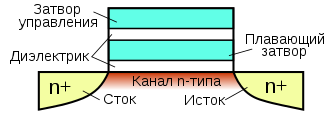
\includegraphics[scale=0.8]{floating_gate_transistor.png}
    }
    \caption{Транзистор с плавающим затвором}\label{fig:floating_gate_transistor}
\end{figure}

Стоит отметить, что в большинстве современных устройств флеш-памяти используются многобитовые ячейки памяти (multi-level cell), которые позволяют увеличить объём хранимой информации за счёт увеличения количества различимых состояний заряда на затворе (\(2^N\) состояний соответствуют \(N\) битам памяти).

Для повышения объёма записи в данный момент преимущественно используется увеличение количества слоёв в устройстве с помощью перехода к изготовлению трёхмерных интегральных микросхем (3D IC) и 3D V NAND...

Потенциально большая скорость
Открывают ряд преимуществ
- Возможность создания универсальной памяти, сочетающей в себе быстрый доступ к информации и энергонезависимость
- Потенциально неограниченное количество циклов перезаписи
- Потенциально большая скорость

\section{Сегнетоэлектрическая память}\label{sec:ch0/sec2}
\subsection{Сегнетоэлектрики}
Сегнетоэлектричество (СЭ) "--- свойство материалов, позволяющее им обладать спонтанной поляризацией. То есть в отсутствии внешнего электрического поля в таких веществах сохраняется ненулевой вектор поляризации. Наличие этого свойства в материале определяется кристаллической решёткой. Так, СЭ может проявляться лишь в таких пространственных группах (фазах) вещества, кристаллическая решётка (сингония) которых не является центросимметричной.

Одним из наиболее характерных свойств СЭ материалов является наличие петли гистерезиса в зависимости поляризации \(P\) от напряжённости электрического поля \(E\) (рис. \cref{fig:hysteresis}). Важные характеристики, которые часто используются при характеризации СЭ материалов: коэрцитивное поле и остаточная поляризация также отражены на рисунке \cref{fig:hysteresis} Стоит отметить, что зависимость такого вида может быть получена и в несегнетоэлектрических материалах за счёт зарядки/разрядки ловушек в диэлектрике, а значит не может быть использована как критерий проявления СЭ в материалах.

\begin{figure}[ht]
    \centerfloat{
        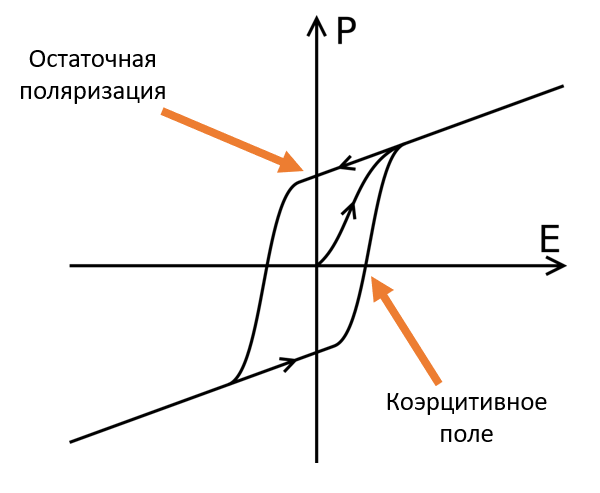
\includegraphics[scale=0.8]{hysteresis.png}
    }
    \caption{Зависимость поляризации \(P\) от напряжённости электрического поля \(E\) в сегнетоэлектрике}\label{fig:hysteresis}
\end{figure}

\subsection{Устройства памяти на основе сегнетоэлектриков}
Наличие двух стабильных состояний кристаллической решётки, которым соответствует положительная и отрицательная поляризация материала позволяет использовать сегнетоэлектрические материалы как функциональный слой в устройствах энергонезависимой памяти. Основные концепции сегнетоэлектрической памяти включают в себя коммерчески доступную сегнетоэлектрическую память с произвольным доступом (ferroelectric random access memory, FRAM), сегнетоэлектрический полевой транзистор (ferroelectric field-effect transistor, FeFET) и сегнетоэлектрический туннельный переход (ferroelectric tunnel junction, FTJ), принципиальная схема которых отражена на рисунке \cref{fig:fram}.

\begin{figure}[ht]
    \centerfloat{
        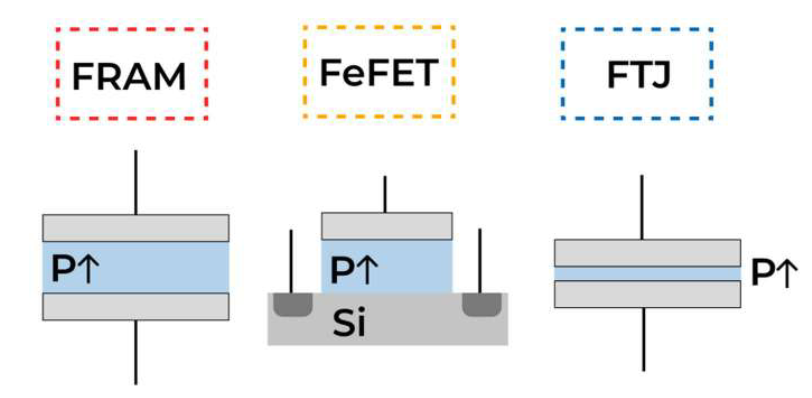
\includegraphics[scale=0.8]{FRAM.png}
    }
    \caption{Схема сегнетоэлектрической памяти}\label{fig:fram}
\end{figure}

\FloatBarrier
           % Глава 1
\chapter{Энергонезависимая память на основе сегнетоэлектрических материалов}\label{ch:ch1}
\section{Флеш-память}\label{sec:ch1/sec1}
На момент написания этой работы доминирующим на рынке видом энергонезависимой памяти (NVM) является флеш-память. Основным компонентом флеш-памяти является транзистор с плавающим затвором (рис. \cref{fig:floating_gate_transistor}). При приложении потенциала к управляющему затвору происходит туннелирование электронов сквозь диэлектрической слой, что приводит к инжекции заряда в плавающий затвор и обеспечивает запись информации в устройстве. При считывании прикладывается напряжение между стоком и истоком, проводимость канала транзистора при этом определяется наличием заряда на плавающем затворе: в отсутствии заряда ток протекает, а при наличии заряда канал остаётся закрытым.

При отсутствии напряжения на плавающем затворе ток через диэлектрик значительно уменьшается, тем самым обеспечивая длительное хранение заряда в затворе, а значит и долгий срок хранения информации в устройстве.

\begin{figure}[ht]
    \centerfloat{
        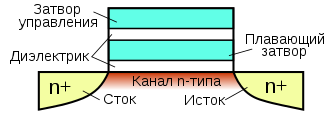
\includegraphics[scale=0.8]{floating_gate_transistor.png}
    }
    \caption{Транзистор с плавающим затвором}\label{fig:floating_gate_transistor}
\end{figure}

Стоит отметить, что в большинстве современных устройств флеш-памяти используются многобитовые ячейки памяти (multi-level cell), которые позволяют увеличить объём хранимой информации за счёт увеличения количества различимых состояний заряда на затворе (\(2^N\) состояний соответствуют \(N\) битам памяти).

Кроме того, для повышения объёма записи в данный момент используется увеличение количества слоёв с ячейками памяти в чипе (3D NAND), а также технология трёхмерной интегральной микросхемы (3D IC), позволяющая упаковывать несколько чипов в одном устройстве.

\section{Сегнетоэлектрическая память}\label{sec:ch1/sec2}
\todo{добавь, зачем заменять флеш, неубедительно, характеристики растут}

\noindent По сравнению с флеш-памятью, сегнетоэлектрическая память обладает рядом потенциальных преимуществ:
\begin{itemize}
    \item Более низкое энергопотребление при записи.
    \item Более высокая скорость записи.
    \item Большее количество циклов перезаписи.
    \item Возможность создания <<универсальной>> памяти, сочетающей в себе скорость работы памяти с произвольным доступом (DRAM) и энергонезависимость.
\end{itemize}

\todo{В связи с этим ведутся разработки бла-бла, мб упомянуть ReRAM, MRAM, etc., если в тему будет, мб section переименовать}
\subsection{Сегнетоэлектрики}
Сегнетоэлектричество (СЭ) "--- свойство материалов, позволяющее им обладать спонтанной поляризацией. То есть в отсутствии внешнего электрического поля в таких веществах сохраняется ненулевой вектор поляризации. Наличие этого свойства в материале определяется кристаллической решёткой. Так, СЭ может проявляться лишь в таких пространственных группах (фазах) вещества, кристаллическая решётка (сингония) которых не является центросимметричной.

Одним из наиболее характерных свойств СЭ материалов является наличие петли гистерезиса в зависимости поляризации \(P\) от напряжённости электрического поля \(E\) (рис. \cref{fig:hysteresis}). Важные характеристики, которые часто используются при характеризации СЭ материалов: коэрцитивное поле и остаточная поляризация также отражены на рисунке \cref{fig:hysteresis}. Стоит отметить, что зависимость такого вида может быть получена и в несегнетоэлектрических материалах за счёт зарядки/разрядки ловушек в диэлектрике, а значит не может быть использована как критерий проявления СЭ в материалах.

\begin{figure}[ht]
    \centerfloat{
        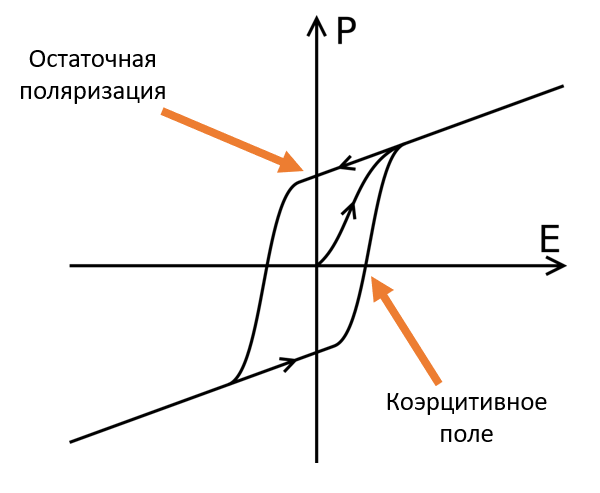
\includegraphics[scale=0.8]{hysteresis.png}
    }
    \caption{Зависимость поляризации \(P\) от напряжённости электрического поля \(E\) в сегнетоэлектрике}\label{fig:hysteresis}
\end{figure}

\subsection{Устройства памяти на основе сегнетоэлектриков}
Наличие двух стабильных состояний кристаллической решётки, которым соответствует положительная и отрицательная поляризация материала (рис. позволяет использовать сегнетоэлектрические материалы как функциональный слой в устройствах энергонезависимой памяти. Основные концепции сегнетоэлектрической памяти включают в себя коммерчески доступную сегнетоэлектрическую память с произвольным доступом (ferroelectric random access memory, FRAM), сегнетоэлектрический полевой транзистор (ferroelectric field-effect transistor, FeFET) и сегнетоэлектрический туннельный переход (ferroelectric tunnel junction, FTJ), принципиальные схемы которых отражены на рисунке \cref{fig:fram}.
\todo{Не знаю куда вставить
    К основным недостаткам FRAM можно отнести низкую плотность записи, по причине необходимости создания структур один транзистор -- один конденсатор (1T-1C); невозможность хранения более одного бита в ячейке, поскольку вектор поляризации, напрямую определяющий значение бита, может находиться лишь в двух состояниях; а также деструктивность считывания.}

\begin{figure}[ht]
    \centerfloat{
        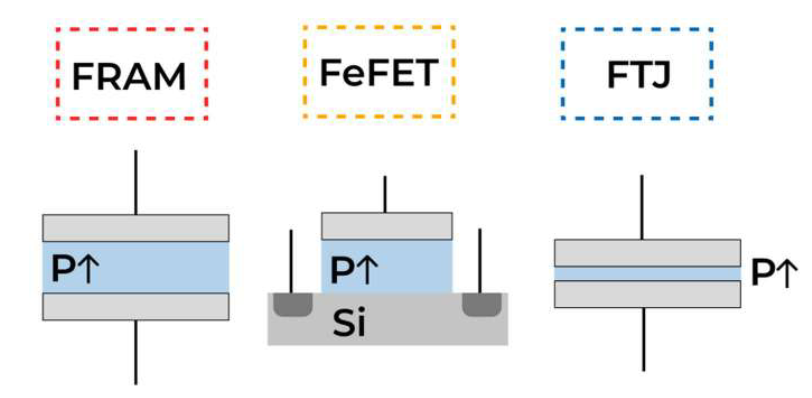
\includegraphics[scale=0.8]{FRAM.png}
    }
    \caption{Схемы концепций сегнетоэлектрической памяти}\label{fig:fram}
\end{figure}

\FloatBarrier
           % Глава 1
\chapter{Методы исследования сегнетоэлектрических конденсаторов}\label{ch:ch2}

\section{Атомно-силовая микроскопия}\label{sec:ch2/sect1}
Атомно-силовая микроскопия (АСМ) позволяет осуществлять картирование рельефа поверхности образца, а также отклика различной природы с высоким пространственным разрешением. Сканирование осуществляется с помощью иглы с радиусом закругления \(\sim\)\SI{10}{\nm}, расположенной на конце кантилевера (рис. \cref{fig:afm_cantilever}). Отклонение кантилевера при взаимодействии иглы с образцом вызывает смещение лазерного луча, отражающегося от поверхности кантилевера, которое, в свою очередь, детектируется при помощи четырёхсекционного фотоприёмника (рис. \cref{fig:afm_system}).

\begin{figure}[ht]
    \centerfloat{
        \hfill
        \subcaptionbox[List-of-Figures entry]{\label{fig:afm_cantilever} Чип, содержащий кантилевер}{%
            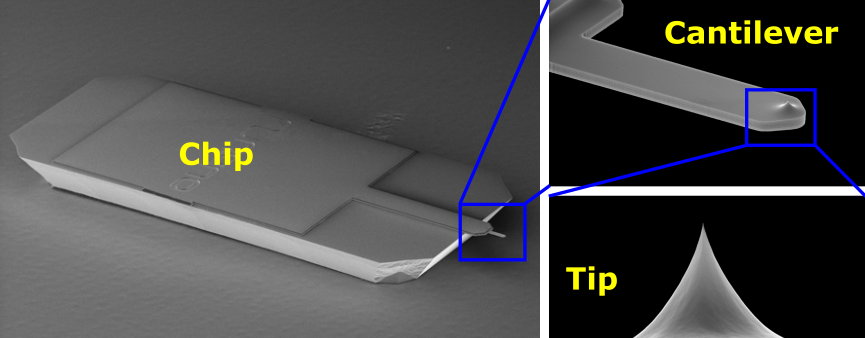
\includegraphics[width=0.5\linewidth]{afm/cantilever.png}}
        \hfill
        \subcaptionbox{\label{fig:afm_system} Оптическая система, детектирующая отклонение кантилевера}{%
            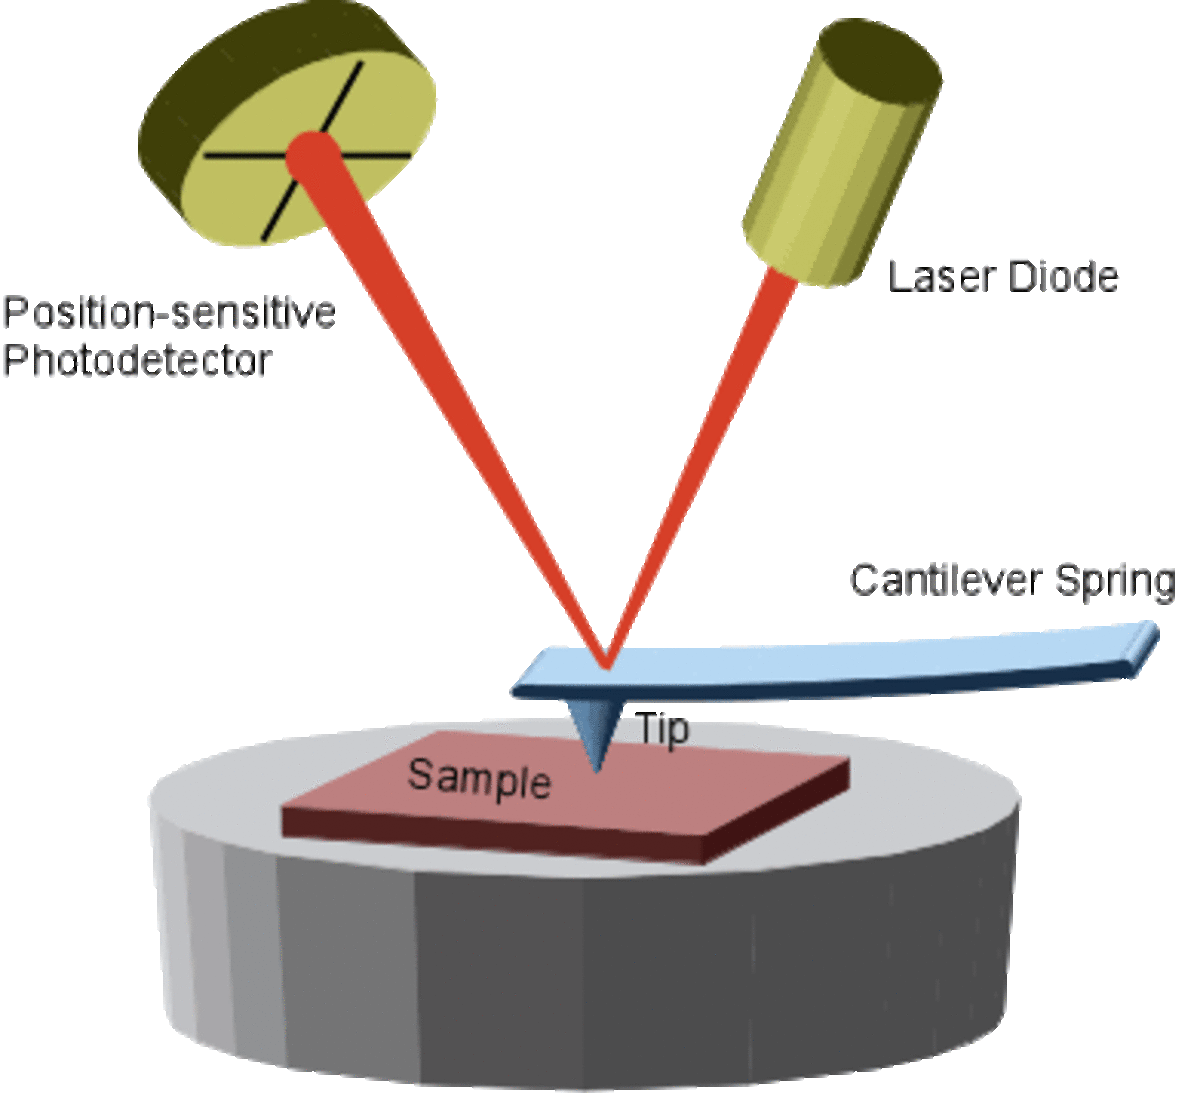
\includegraphics[width=0.5\linewidth]{afm/afm.png}}
        \hfill
    }
    \caption[Этот текст попадает в названия рисунков в списке рисунков]{Базовые принципы атомно-силовой микроскопии}\label{fig:afm}
\end{figure}

\subsection{Микроскопия пьезоотклика}\label{sec:ch2/sect1/sub1}
Микроскопия пьезоотклика (piezoresponse force microscopy, PFM) позволяет исследовать распределение пьезоотклика в пьезоэлектрике с помощью измерения величины деформации, вызванной обратным пьезоэффектом (рис. \cref{fig:pfm}).

\begin{figure}[ht]
    \centerfloat{
        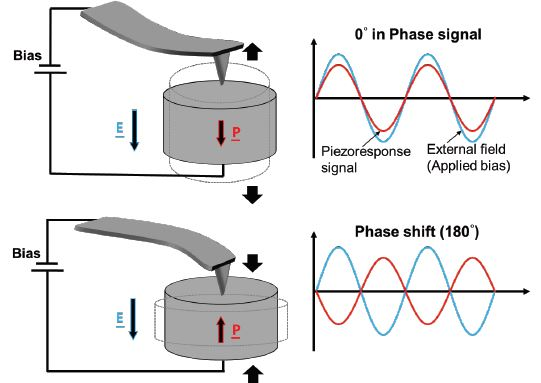
\includegraphics[width=0.6\linewidth]{pfm/pfm.jpg}
    }
    \caption{Микроскопия пьезоотклика}\label{fig:pfm}
\end{figure}

При этом возможно использование двух принципиально разных способов измерения: исследование пьезоотклика сегнетоэлектрического слоя при приложении напряжения между иглой и нижним электродом (\textit{ex citu}\todo{, рис X.Xа, нужно самому нарисовать, в solidworks например, если будешь успевать до защиты}) и исследование пьезоотклика в готовой ячейке памяти (\textit{in situ}, \todo{рис X.Xб}) при приложении напряжения между верхним и нижним электродами. При этом в случае \textit{ex citu} измерений сканируется непосредственно сегнетоэлектрическая плёнка, а в случае \textit{in situ} измерений сканируется поверхность электрода, деформирующаяся вслед за сегнетоэлектрическим слоем. Каждый из подходов имеет свои недостатки и преимущества. Так, в случае \textit{ex situ} измерений возможно \todo{протекание электрохимических реакций на поверхности сегнетоэлектрика [ref], неравномерное электрическое поле, которое к тому же в значительной степени зависит от формы иглы в момент измерения, возможно контролируемое зарождение домена с обратной поляризацией в месте контакта с зондом}, однако \textit{in situ} измерения неизбежно ухудшают пространственное разрешение ...,

\todo{Из-за слабого отклика появляется необходимость в использовании резонансных методик, а поскольку контактная резонансная частота изменяется при сканировании поверхности, возникает необходимость отслеживания резонансной частоты при измерениях, DART, BE PFM сравнение}

\todo{Для получения амплитуды и фазы отклика используется Фурье преобразование сигнала с фотоприёмника, после чего полученный спектр фильтруется и с помощью алгоритма vector fitting аппроксимируется для получения амплитуды и фазы отклика на резонасной частоте, по-хорошему сюда бы ещё картинку сырые данные -> fft -> filtered fft -> vector fit, мб у Калинина или у нас в статьях есть}

\subsubsection{Измерение латерального пьезоотклика}
При использовании АСМ возможно детектирование не только вертикального отклонения кантилевера, но и его изгиба относительно своей оси. Это имеет особый интерес в случае PFM измерений, поскольку позволяет получить латеральный пьезоотклик структуры \todo{рисунок}. При этом при получении карты вертикального отклика, а также карт латерального отклика в \todo{обычном} положении и при повороте образца на \ang{90}, возможно восстановить распределение трёхмерного вектора отклика, а значит и полного вектора поляризации. \todo{объяснить, зачем поворот нужен}

Однако, для количественного сопоставления карт вертикального и латерального откликов необходимо провести дополнительную калибровочную процедуру. Кроме стандартного перевода сигнала, соответствующего вертикальному отклонению кантилевера, в вертикальный пьезоотклик, необходимо получить соотношение, связывающее величины вертикального и латерального отклонений кантилевера. Для этого предлагается следующая методика: сканирование проводится в области, содержащей границу между СЭ и неСЭ областями, при этом в каждой точке измеряется как вертикальная, так и латеральная величина отклонения кантилевера. На границе СЭ области при этом будет наблюдаться некоторый пьезоотклик, однако, благодаря эффекту Пуассона вертикальное растяжение слоя HZO также вызовет его локальное сжатие в направлении, поперечном границе областей. Это приведёт к смещению слоя со стороны неСЭ области, а значит будет вызывать отклонение кантилевера, соответствующее латеральному пьезоотклику, несмотря на отсутствие отклика в неСЭ области.

Для подтверждения теоретических соображений было проведено моделирование методом конечных элементов в среде COMSOL. Использованная геометрия приведена на рис. \cref{fig:comsol:geometry}. Были использованы физические характеристики материалов Si, W, HfO\(_2\), Pt из библиотеки материалов COMSOL. Для упрощения модели пьезоотклик HfO\(_2\) был смоделирован с помощью механических напряжений на границе СЭ области с размером в \SI{100}{\nano\meter}, которая была расположена в центре неСЭ области. При моделировании использовалась свободная треугольная сетка, генерируемая по умолчанию. Полученные распределения вертикального и латерального пьезоотклика показаны на рис. \cref{fig:comsol:vertical} и \cref{fig:comsol:lateral} соответственно. Абсолютный вертикальный отклик при этом оказался больше латерального в \(\frac{\Delta h}{\Delta w}\sim\) 4-5 раз в зависимости от толщины электрода. Для относительных величин получаем \(\frac{\Delta w}{w} = \nu \frac{\Delta h}{h}\)

\begin{figure}[ht]
    \centerfloat{
        \hfill
        \subcaptionbox[List-of-Figures entry]{\label{fig:comsol:geometry} Геометрия модели}{%
            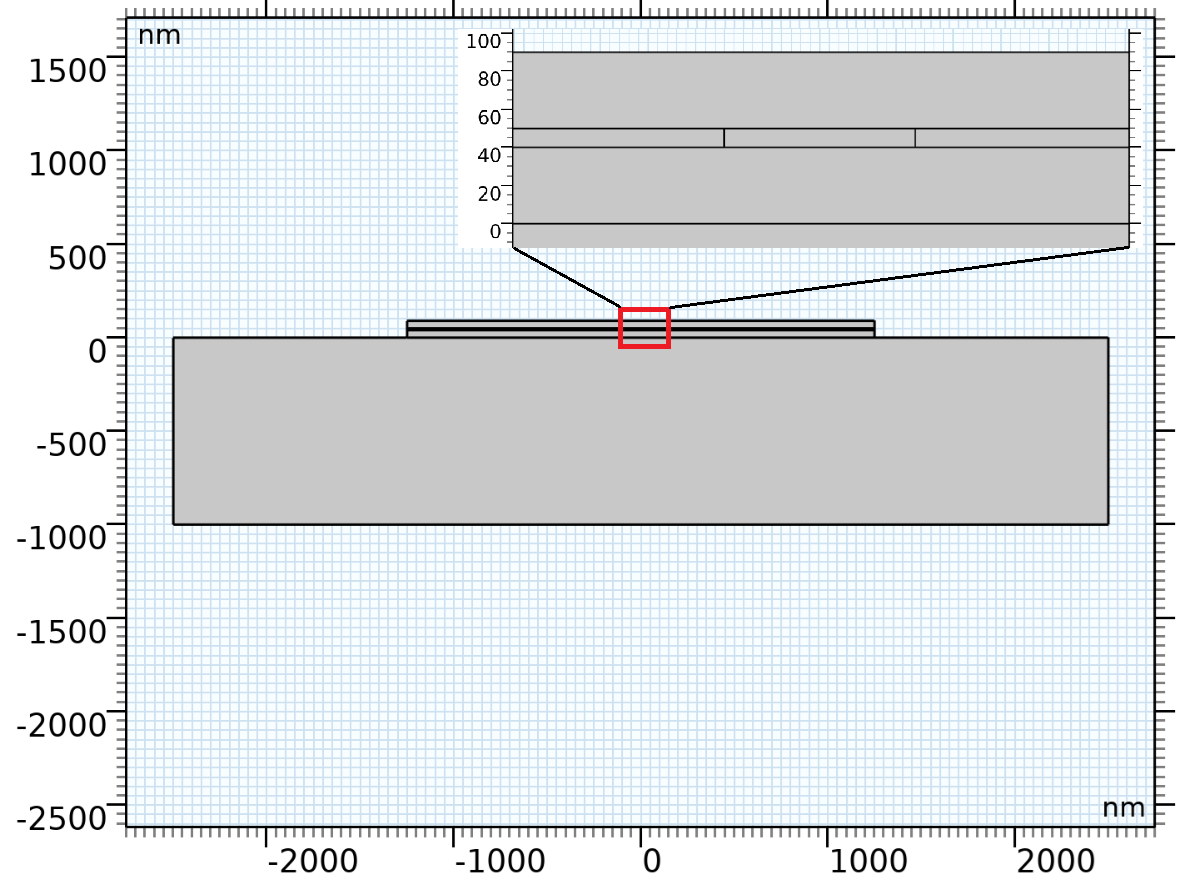
\includegraphics[width=0.33\linewidth]{comsol/geometry.png}}
        \hfill
        \subcaptionbox{\label{fig:comsol:vertical} Вертикальный отклик}{%
            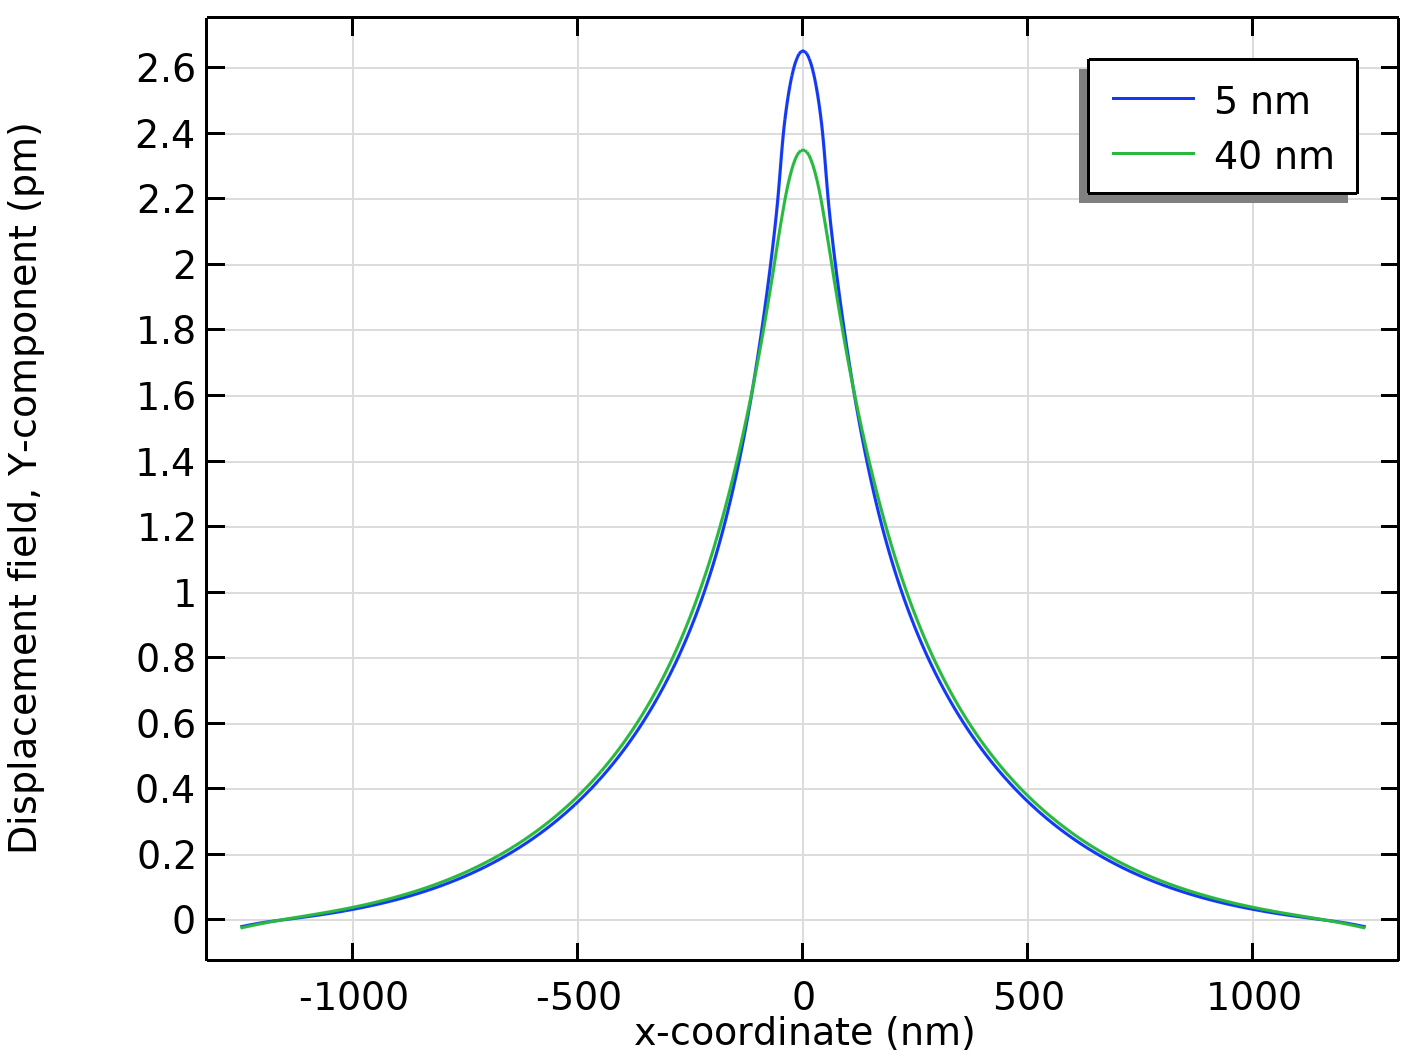
\includegraphics[width=0.33\linewidth]{comsol/vertical.png}}
        \hfill
        \subcaptionbox{\label{fig:comsol:lateral} Латеральный отклик}{%
            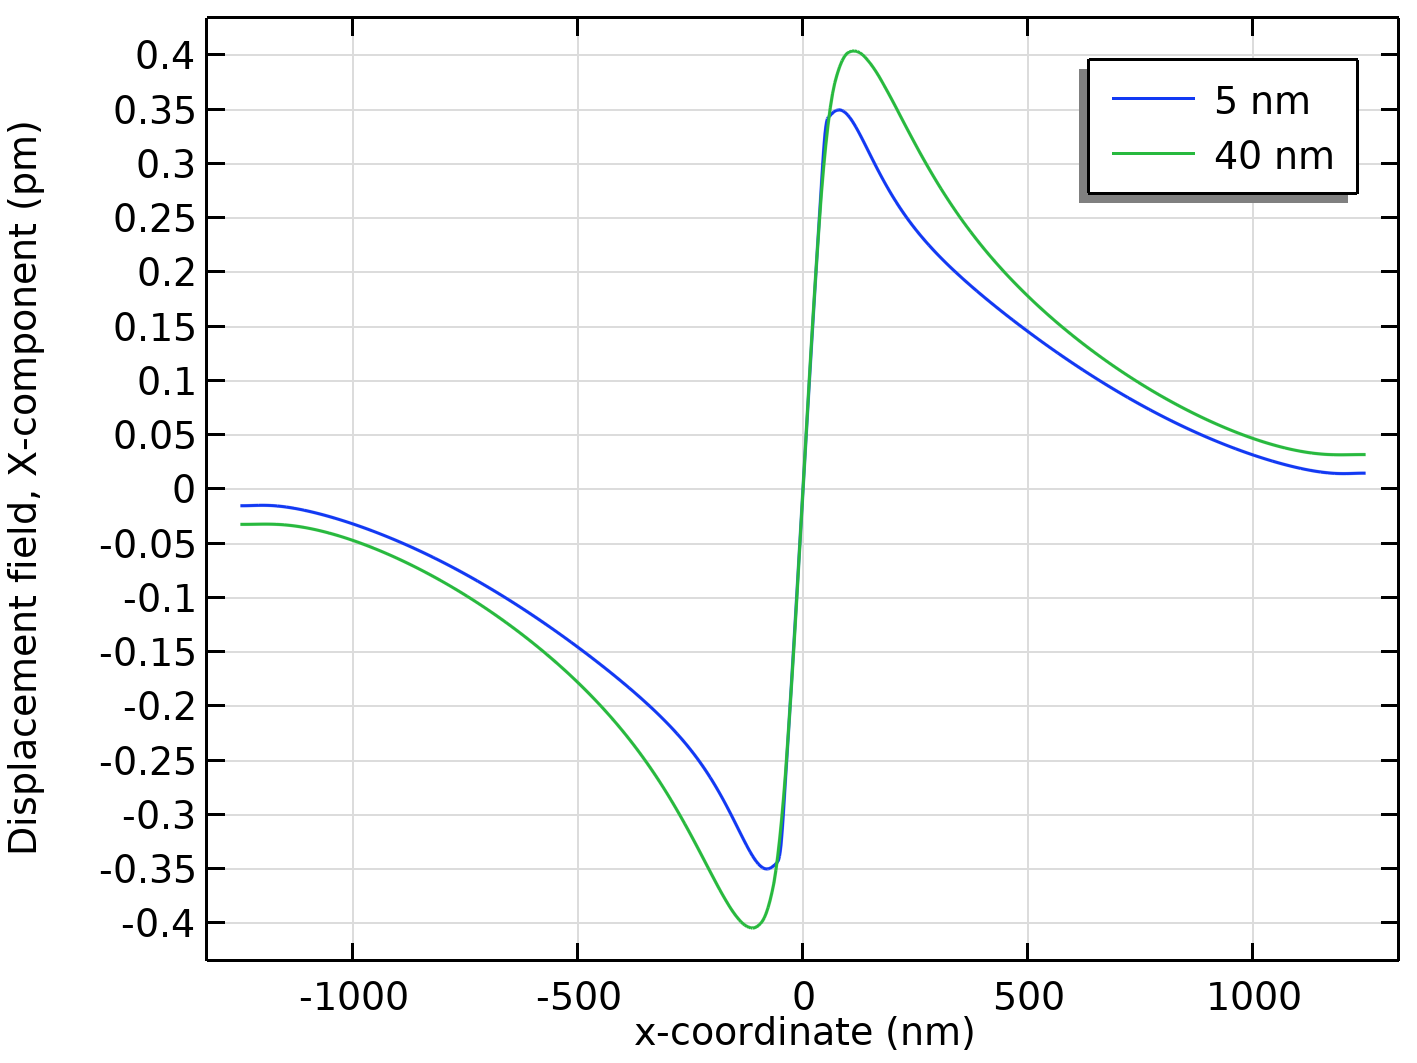
\includegraphics[width=0.33\linewidth]{comsol/lateral.png}}
        \hfill
    }
    \caption[Этот текст попадает в названия рисунков в списке рисунков]{Моделирование пьезоотклика на границе сегнетоэлектрической и несегнетоэлектрической фазы методом конечных элементов при различной толщине верхнего электрода}\label{fig:comsol}
\end{figure}

Используя полученное отношение можно перевести амплитуду латерального отклика в те же единицы, которые используются для вычисления амплитуды вертикального отклика:

\[A_y = \nu A_z\]
\todo{
    % \subsubsection{Спектроскопия}
    % (Switching spectroscopy, SS PFM)

    % \subsubsection{Количественные измерения}
    % Для получения количественных результатов при PFM измерениях необходимо провести калибровку \todo{прибора, кантилевер}. Для этого используется \todo{возбуждение кантилевера в воздухе} ... термопик

    % \section{Электрофизические измерения}
    % Зондовая станция, PUND, CV, PQ (написать какие импульсы подаются, рисуночек, особенно для PQ, объяснить токи)

}           % Глава 2
% \chapter{Сегнетоэлектрические материалы}\label{ch:ch3}

\section{Моделирование процесса напыления}\label{sec:ch3/sec2}
% Для бла-бла было произведено моделирование 
Для моделирования взаимодействия налетающих частиц платины с HZO были произведены квантовомеханические расчёты столкновений на основе метода Монте-Карло с помощью пакета Stopping and Range of Ions in Matter (SRIM) \cite{zieglerSRIMStoppingRange2010}. Оценка энергии налетаемых частиц была получена с помощью расчёта кинетической энергии атомов при лазерной абляции \cite{mutaevVLIYaNIEVERHNEYGRANICY2020}:
\todo{добавить интуиции к формулке}
\[\bar{E} = 9.92 \cdot 10^{4} A^{1/8} \tau^{1/4} Z^{3/4} (Z+1)^{3/8} (I\lambda)^{1/2}k_b,\] где \(A\) -- атомная масса распыляемого элемента, \(\tau\) -- длительность импульса, \(Z\) -- средний заряд ионов, вылетающих при абляции, \(I\) -- интенсивность лазерного излучения в \si{\watt}/\si{\cm}\(^2\), \(\lambda\) -- длина волны лазера, \(k_b\) -- постоянная Больцмана.

При импульсном лазерном напылении использовался лазер Nd:YAG с длиной волны \(\lambda=\) \SI{1064}{\nano\meter}, длительностью импульсов \(\tau=\) \SI{10}{\nano\second}. Интенсивность оценивалась как \(I=\alpha(1-\beta)\frac{J}{S}\), где \(\alpha=(1-R)^{2N}\) -- коэффициент прохождения излучения через \(N=5\) элементов оптической системы, изготовленных из кварцевого стекла с отражательной способностью \(R=0.0337\) \cite{polyanskiyRefractiveindexInfoDatabase2024} для длины волны \(\lambda\) (поглощение при этом не учитывалось), \(\beta=0.748\) -- отражательная способность платины \cite{weberHandbookOpticalMaterials2003}, \(J\) -- энергия одного импульса, \(S\) -- площадь лазерного пятна. Для оценки также использовался характерный средний заряд ионов Pt при лазерном напылении $Z=0.56$ \cite[с.~141]{easonPulsedLaserDeposition2007}

\begin{table} [htbp]
    \centering
    \begin{threeparttable}% выравнивание подписи по границам таблицы
        \caption{Название таблицы}\label{tab:Ts0Sib}%
        \begin{tabular}{ | p{2.5cm} | p{3cm} | p{3cm} | p{2.3cm}l | }
            \hline
            \hline
            \centering \(J\), \si{\milli\joule} & \centering \(I\), \si{\giga\watt}/\si{\cm}\(^2\) & \centering \(\bar{E}\), \si{\electronvolt} & \centering \(d\), \si{\nm} & \\
            \hline
            \centering 225                      & \centering  13.4                                 & \centering  151                            & \centering  1.3            & \\
            \centering 145                      & \centering  8.6                                  & \centering  121                            & \centering 1.2             & \\
            \centering 93                       & \centering  5.5                                  & \centering  97                             & \centering 1.1             & \\
            \centering 45                       & \centering  2.7                                  & \centering  68                             & \centering 1.0             & \\
            \hline
            \hline
        \end{tabular}
    \end{threeparttable}
\end{table}

На рисунке \cref{fig:pt_distr} показано \todo{вероятностное} распределение атомов платины в слое HZO при \todo{... многократном} ... Стоит отметить, что при распылении проникновение частиц платины в HZO быстро заканчивается: расстояние между плоскостями (111) в кубической гранецентрированной решётке составляет \(\frac{a}{\sqrt{3}}\approx\) \SI{2.26}{\angstrom}, поэтому структурные свойства HZO могут измениться лишь при напылении \(\sim 4-5\) первых атомных слоёв.

\begin{figure}[ht]
    \centerfloat{
        \hfill
        \subcaptionbox[List-of-Figures entry]{\label{fig:pt_distr_151eV} \SI{151}{\electronvolt}}{%
            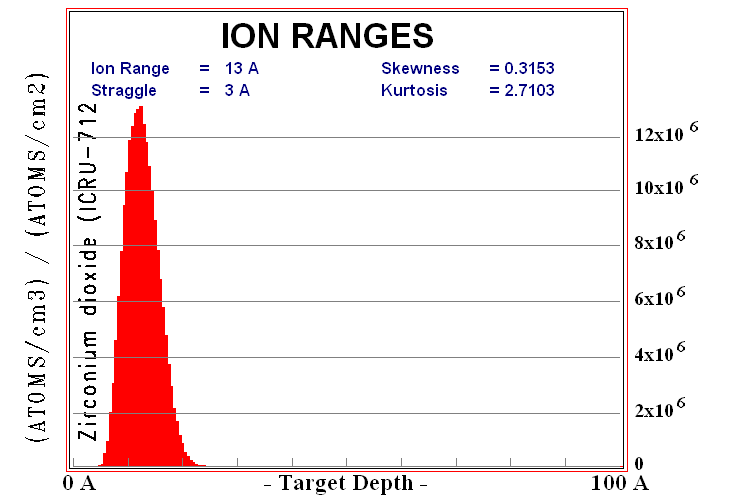
\includegraphics[width=0.5\linewidth]{151 eV.png}}
        \hfill
        \subcaptionbox{\label{fig:pt_distr_121eV}\SI{121}{\electronvolt}}{%
            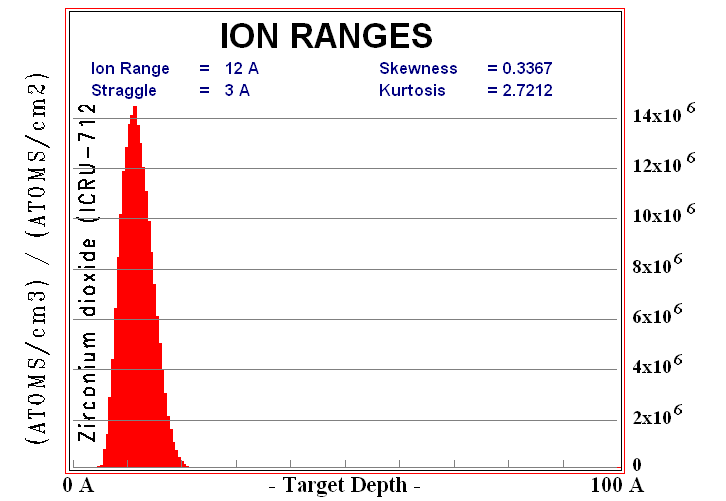
\includegraphics[width=0.5\linewidth]{121 eV.png}}
        \hfill
        \\
        \subcaptionbox{\label{fig:pt_distr_97eV}\SI{97}{\electronvolt}}{%
            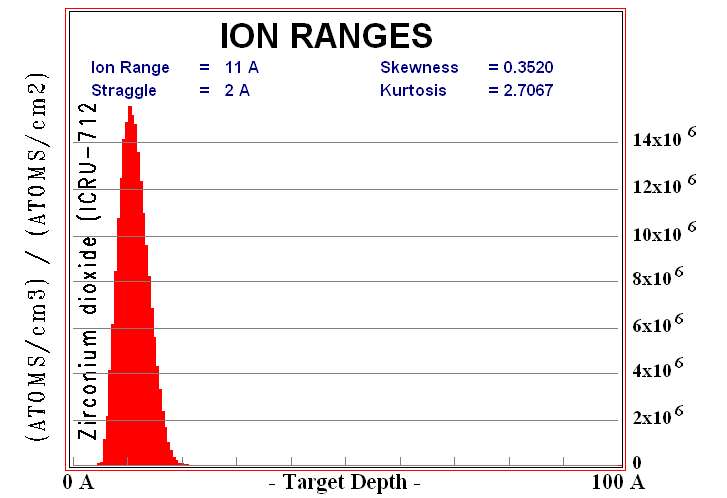
\includegraphics[width=0.5\linewidth]{97 eV.png}}
        \hfill
        \subcaptionbox{\label{fig:pt_distr_68eV}\SI{68}{\electronvolt}}{%
            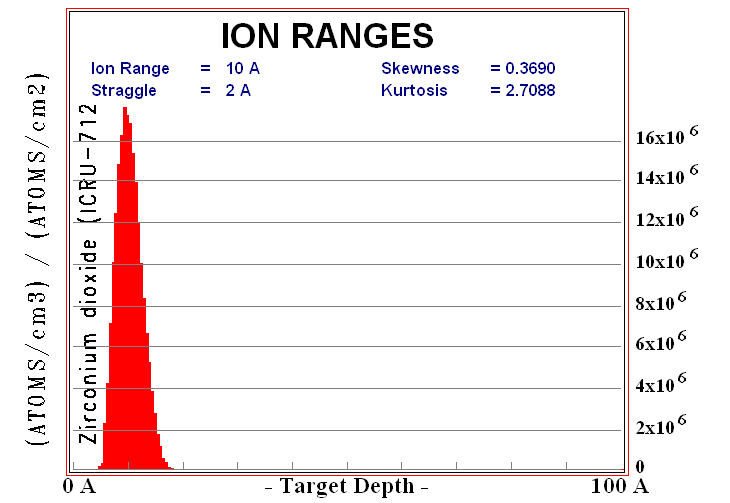
\includegraphics[width=0.5\linewidth]{68 eV.png}}
        \hfill
    }
    \caption[Этот текст попадает в названия рисунков в списке рисунков]{Распределение атомов платины в плёнке HZO \todo{после 100 000 актов распыления} при различных энергиях распыляемых частиц}\label{fig:pt_distr}
\end{figure}

\nomenclature{FEM}{finite element method, метод конечных элементов}
\nomenclature{HZO}{Hf0.5Zr0.5O2, оксид гафния-циркония}
\nomenclature{АСО}{атомно-слоевое осаждение}
\nomenclature{АСМ}{атомно-силовая микроскопия}
\nomenclature{PUND}{positive up negative down, электрофизический метод измерения остаточной поляризации}
\nomenclature{CMOS}{complementary metal-oxide-semiconductor, комплементарная структура металл-оксид-полупроводник}
\nomenclature{БТО}{быстрая термическая обработка}
\nomenclature{NVM}{non-volatile memory, энергонезависимая память}
\nomenclature{FIT}{finite integration technique, метод конечных интегралов}
\nomenclature{FMM}{fast multipole method, быстрый метод многополюсника}
\nomenclature{FVTD}{finite volume time-domain, метод конечных объёмов
    во~временной области}
\nomenclature{MLFMA}{multilevel fast multipole algorithm, многоуровневый
    быстрый алгоритм многополюсника}
\nomenclature{BEM}{boundary element method, метод граничных элементов}
\nomenclature{CST MWS}{Computer Simulation Technology Microwave Studio
    программа для компьютерного моделирования уравнен Максвелла}
\nomenclature{DDA}{discrete dipole approximation, приближение дискретиных
    диполей}

\FloatBarrier
           % Глава 3
\chapter*{Заключение}                       % Заголовок
\addcontentsline{toc}{chapter}{Заключение}  % Добавляем его в оглавление

%% Согласно ГОСТ Р 7.0.11-2011:
%% 5.3.3 В заключении диссертации излагают итоги выполненного исследования, рекомендации, перспективы дальнейшей разработки темы.
%% 9.2.3 В заключении автореферата диссертации излагают итоги данного исследования, рекомендации и перспективы дальнейшей разработки темы.
%% Поэтому имеет смысл сделать эту часть общей и загрузить из одного файла в автореферат и в диссертацию:

%% Согласно ГОСТ Р 7.0.11-2011:
%% 5.3.3 В заключении диссертации излагают итоги выполненного исследования, рекомендации, перспективы дальнейшей разработки темы.
%% 9.2.3 В заключении автореферата диссертации излагают итоги данного исследования, рекомендации и перспективы дальнейшей разработки темы.
В работе было проведено исследование возможных физических механизмов, влияющих на сегнетоэлектрические свойства конденсаторов на основе оксида гафния-циркония. На примере исследования микроскопических и функциональных свойств структур W/Hf\(_{0.5}\)Zr\(_{0.5}\)O\(_2\)/Pt методами АСМ, РЭМ, XRD, PFM и электрофизическими измерениями было показано, что параметры, используемые при импульсном лазерном напылении, могут существенно влиять на функциональные свойства ячеек сегнетоэлектрической памяти.

В ходе работы были получены следующие экспериментальные результаты: установлено, что в структурах, изготовленных при напылении платинового электрода лазерными импульсами большей энергии, наблюдается увеличение размера доменов, уменьшение величины встроенного электрического поля и увеличение остаточной поляризации. Физический механизм, объясняющий экспериментальные результаты, связан с влиянием размера зёрен платины, который увеличивается при увеличении энергии импульсов. Увеличение размера зёрен приводит к уменьшению длины границ зёрен, которые являются резервуаром для сегрегации атомов кислорода оксида гафния-циркония и через которые также возможна миграция атомов кислорода в окружающую среду. В результате, увеличение размера зёрен платины приводит к уменьшению плотности заряженных вакансий и величины диполя на верхней границе раздела, что в свою очередь уменьшает встроенное электрическое поле в пленке оксида гафния-циркония. Как известно, встроенное поле может значительно изменять сегнетоэлектрические свойства структур, в частности приводя к различной выраженности эффекта wake-up и различным значениям величины остаточной поляризации.

Кроме того, в работе был предложен метод для количественного сравнения вертикальной и латеральной компоненты пьезоотклика при измерениях с помощью микроскопии пьезоотклика. Метод был использован для восстановления трёхмерного вектора поляризации в функциональной структуре на основе оксида гафния. Было показано, что при переключении поляризации в большей части структуры происходит поворот вектора поляризации на \ang{180}, что объясняется наличием одной полярной оси в структурной орторомбической фазе \(Pca2_1\). Однако также наблюдаются области ферроупругого переключения, в которых поляризация переключается не на \ang{180}, что объясняется локальными механическими напряжениями, сохраняющимися даже после проведения процедуры электротренировки. Кроме того, установлено, что латеральный пьезоэлектрический отклик превышает вертикальный, что говорит о перспективности применения данного материала для разработки устройств на основе гетероструктур ферромагнетик-сегнетооэлектрик, принцип действия которых основан на обратном магнитострикционнном эффекте. Таким образом, предложенный метод может быть полезным как в исследовании природы сегнетоэлектрических свойств в новых материалах, так и в более прикладных задачах.



В заключение автор выражает благодарность своему научному руководителю А.\,А.~Чуприк за помощь в выборе тематики исследований, трактовке полученных экспериментальных результатов, а также за всяческую поддержку в течение работы в лаборатории. Также автор благодарит И.\,А.~Савичева за помощь в погружении в исследуемую область в начале своего пути и за обсуждение различных вопросов, возникавших в течение научной деятельности. Автор  благодарит М.\,В.~Спиридонова за помощь в освоении микроскопии пьезоотклика и устранении различных технических неполадок, возникавших в ходе экспериментов, и И.\,А.~Мутаева за изготовление исследуемых образцов, проведение XRD и РЭМ экспериментов и обсуждение физики процессов импульсного лазерного осаждения.
      % Заключение
\include{Dissertation/acronyms}        % Список сокращений и условных обозначений
% \include{Dissertation/dictionary}      % Словарь терминов
\include{Dissertation/references}      % Список литературы
% \include{Dissertation/lists}           % Списки таблиц и изображений (иллюстративный материал)

\setcounter{totalchapter}{\value{chapter}} % Подсчёт количества глав

%%% Настройки для приложений
\appendix
% Оформление заголовков приложений ближе к ГОСТ:
\setlength{\midchapskip}{20pt}
\renewcommand*{\afterchapternum}{\par\nobreak\vskip \midchapskip}
\renewcommand\thechapter{\Asbuk{chapter}} % Чтобы приложения русскими буквами нумеровались

\include{Dissertation/appendix}        % Приложения

\setcounter{totalappendix}{\value{chapter}} % Подсчёт количества приложений

\end{document}
